%%%%%%%%%%%%%%%%%%%%%%%%%%%%%%%%%%%%%%%%%
% Masters/Doctoral Thesis 
% LaTeX Template
% Version 2.4 (22/11/16)
%
% This template has been downloaded from:
% http://www.LaTeXTemplates.com
%
% Version 2.x major modifications by:
% Vel (vel@latextemplates.com)
%
% This template is based on a template by:
% Steve Gunn (http://users.ecs.soton.ac.uk/srg/softwaretools/document/templates/)
% Sunil Patel (http://www.sunilpatel.co.uk/thesis-template/)
%
% Template license:
% CC BY-NC-SA 3.0 (http://creativecommons.org/licenses/by-nc-sa/3.0/)
%
%%%%%%%%%%%%%%%%%%%%%%%%%%%%%%%%%%%%%%%%%

%----------------------------------------------------------------------------------------
%	PACKAGES AND OTHER DOCUMENT CONFIGURATIONS
%----------------------------------------------------------------------------------------

\documentclass[
12pt, % The default document font size, options: 10pt, 11pt, 12pt
%oneside, % Two side (alternating margins) for binding by default, uncomment to switch to one side
english, % ngerman for German
onehalfspacing, % Single line spacing, alternatives: singlespacing onehalfspacing or doublespacing
%draft, % Uncomment to enable draft mode (no pictures, no links, overfull hboxes indicated)
%nolistspacing, % If the document is onehalfspacing or doublespacing, uncomment this to set spacing in lists to single
%liststotoc, % Uncomment to add the list of figures/tables/etc to the table of contents
%toctotoc, % Uncomment to add the main table of contents to the table of contents
%parskip, % Uncomment to add space between paragraphs
%nohyperref, % Uncomment to not load the hyperref package
headsepline, % Uncomment to get a line under the header
chapterinoneline, % Uncomment to place the chapter title next to the number on one line
%consistentlayout, % Uncomment to change the layout of the declaration, abstract and acknowledgements pages to match the default layout
]{MastersDoctoralThesis} % The class file specifying the document structure

\usepackage[utf8]{inputenc} % Required for inputting international characters
\usepackage[T1]{fontenc} % Output font encoding for international characters

\usepackage{palatino} % Use the Palatino font by default

%%% Autre packages

\usepackage{tikz}
\usetikzlibrary{mindmap,trees}
\usepackage{epstopdf}

\usepackage{lipsum}
\usepackage{shorttoc}
\usepackage{titletoc}

\usepackage{amsmath}
\usepackage{amssymb}
\usepackage{rotating}
\usepackage{multirow}

\usepackage{float}

\usepackage[lofdepth,lotdepth]{subfig}

\usepackage{indentfirst}
%\setlength{\parindent}{0pt} % remove indent

\usepackage{epstopdf}

\usetikzlibrary{arrows,shapes,snakes,spy,trees,decorations,shadows,positioning}

\usepackage{pgfplots}
\usepackage{pgfplotstable}


%%% Commands

%%% Avoid pages jump (comment for final version)

%\let\cleardoublepageold\cleardoublepage
%\let\clearpageold\clearpage

%\renewcommand{\cleardoublepage}{}
%\renewcommand{\clearpage}{}

%%%

\newcommand{\openchapter}{%\pagebreak
\thispagestyle{empty}
\vspace*{1pt}
\pagebreak
}

\newcommand{\includetex}[1]{\openchapter\include{#1}}

%%%

\usetikzlibrary{arrows,shapes,snakes,spy,trees,decorations,shadows,positioning}
%\usetikzlibrary{shadows}
%\usetikzlibrary{arrows}

%%%

\usepackage{amsmath}
\usepackage{amssymb}
\usepackage{rotating}
\usepackage{multirow}

%%%

\newenvironment{figurethesis}[1]
{
\begin{figure}[htbp]
\begin{center}
}
{
\end{center}
\end{figure}
}
%%%

% Mise en forme Tikz (schéma général + logo lupin)
\definecolor{IGNVert}{RGB}{148, 192,  22}
\definecolor{IGNGris}{RGB}{112, 119, 122}
\definecolor{IGNRouge}{RGB}{255, 100, 100}
\definecolor{IGNFonce}{RGB}{55, 58, 60}


\tikzset{
    myArrowIGNGris/.style={->, >=latex,rounded corners, color = IGNGris, thick,font=\scriptsize},
    myArrowDotIGNGris/.style={->, >=latex, densely dashed, shorten >=1pt, rounded corners, color = IGNGris, thick,font=\scriptsize},
    myArrowIGNRouge/.style={-, >=latex, densely dashed, shorten >=1pt, rounded corners, color = IGNRouge, thick,font=\scriptsize},
    myNodeIGNGris/.style={rectangle,rounded corners,draw=black, top color=white, bottom color=IGNGris!80, inner sep=0.5em, minimum size=0.5em, text centered,font=\normalsize },
    myNodeIGNVert/.style={rectangle,rounded corners,draw=black, top color=white, bottom color=IGNVert!80, inner sep=0.5em, minimum size=0.5em, text centered,font=\normalsize },
    myNodeIGNRouge/.style={rectangle,rounded corners,draw=black, top color=white, bottom color=IGNRouge!80, inner sep=0.5em, minimum size=0.5em, text centered,font=\normalsize },
    myNodeIGNRouge1/.style={rectangle,rounded corners, top color=IGNRouge!50, bottom color=IGNRouge, inner sep=0.5em, minimum size=0.5em, text centered,font=\normalsize }
}

%%% Minitoc

\newcommand\ToCrule{\noindent\rule[5pt]{\textwidth}{1.5pt}}

\newcommand\ToCrulev{\tikz\draw[line width=1.5pt, black] (0,0) arc (110:70:1) arc (-110:-70:1) arc (110:70:1) arc (-110:-70:1) arc (110:70:1) arc (-110:-70:1) arc (110:70:1) arc (-110:-70:1) arc (110:70:1) arc (-110:-70:1) arc (110:70:1) arc (-110:-70:1) arc (110:70:1) arc (-110:-70:1)  arc (110:70:1) arc (-110:-70:1) arc (110:70:1) arc (-110:-70:1) arc (110:70:1);}

\newcommand\ToCruleiv{\tikz\draw[line width=1.5pt, black] (0,0) arc (-110:-70:1) arc (110:70:1) arc (-110:-70:1) arc (110:70:1) arc (-110:-70:1) arc (110:70:1) arc (-110:-70:1) arc (110:70:1) arc (-110:-70:1) arc (110:70:1) arc (-110:-70:1) arc (110:70:1) arc (-110:-70:1)  arc (110:70:1) arc (-110:-70:1) arc (110:70:1) arc (-110:-70:1) arc (110:70:1) arc (-110:-70:1);}


\makeatletter
\newcommand\Mprintcontents{%
  \vspace*{-1cm}
  \vfill
  \begin{center}\ToCrulev\end{center}
  \begin{center}\ttl@printlist[chapters]{toc}{}{1}{}\par\nobreak\end{center}
  \begin{center}\ToCruleiv\end{center}
  \vfill
  \pagebreak}
\makeatother


\newcommand{\keyword}[1]{\textbf{#1}}
\newcommand{\tabhead}[1]{\textbf{#1}}
\newcommand{\code}[1]{\texttt{#1}}
\newcommand{\file}[1]{\texttt{\bfseries#1}}
\newcommand{\option}[1]{\texttt{\itshape#1}}

%%% Colors

\definecolor{t1}{RGB}{255, 0, 0 }
\definecolor{t2}{RGB}{0, 255, 0 }
\definecolor{t3}{RGB}{0, 0, 255 }
\definecolor{t4}{RGB}{255, 255, 0 }
\definecolor{t4}{RGB}{200, 200, 0 }
\definecolor{t4b}{RGB}{200, 200, 0 }
\definecolor{t5}{RGB}{255, 127, 0 }
\definecolor{t6}{RGB}{255, 0, 255 }
\definecolor{t7}{RGB}{0, 255, 255 }
\definecolor{t8}{RGB}{200, 0, 100 }
\definecolor{t9}{RGB}{160, 60, 10 }
\definecolor{t10}{RGB}{0, 160, 160 }
\definecolor{t11}{RGB}{135, 135, 0 }
\definecolor{t12}{RGB}{145, 0, 0 }

\definecolor{l0}{RGB}{000, 000, 000}
\definecolor{l1}{RGB}{255, 000, 000}
\definecolor{l2}{RGB}{000, 255, 000}
\definecolor{l3}{RGB}{000, 000, 255}
\definecolor{l4}{RGB}{255, 255, 000}
\definecolor{l5}{RGB}{255, 000, 255}
\definecolor{l6}{RGB}{000, 255, 255}
\definecolor{l7}{RGB}{255, 127, 000}
\definecolor{l8}{RGB}{255, 000, 127}
\definecolor{l9}{RGB}{127, 255, 000}
\definecolor{l10}{RGB}{000, 255, 127}
\definecolor{l11}{RGB}{127, 000, 255}
\definecolor{l12}{RGB}{000, 127, 255}
\definecolor{l13}{RGB}{127, 000, 000}
\definecolor{l14}{RGB}{000, 127, 000}
\definecolor{l15}{RGB}{000, 000, 127}
\definecolor{l16}{RGB}{127, 127, 000}
\definecolor{l17}{RGB}{127, 000, 127}
\definecolor{l18}{RGB}{000, 127, 127}
\definecolor{l19}{RGB}{127, 127, 127}

%%% Colored shapes

\newcommand{\p[1]}{\tikz\draw[#1,fill=#1] (0,0) circle (1.5mm);}
\newcommand{\li[1]}{\tikz\draw[#1,fill=#1] (0,0) -- (0.25,0) -- (0.25,0.25) -- (0,0.25) -- (0,0);}



\usepackage{indentfirst}
%\setlength{\parindent}{0pt} % remove indent


%%%

\usepackage[maxbibnames=99, maxcitenames=1, backend=bibtex,style=alphabetic-verb,natbib=true]{biblatex} % Use the bibtex backend with the authoryear citation style (which resembles APA)

%\usepackage[maxbibnames=99, maxcitenames=1, backend=bibtex,style=authoryear,natbib=true]{biblatex} % Use the bibtex backend with the authoryear citation style (which resembles APA)

\addbibresource{example.bib} % The filename of the bibliography

\usepackage[autostyle=true]{csquotes} % Required to generate language-dependent quotes in the bibliography

%----------------------------------------------------------------------------------------
%	MARGIN SETTINGS
%----------------------------------------------------------------------------------------

\geometry{
	paper=a4paper, % Change to letterpaper for US letter
	inner=1.0cm, % Inner margin 2.5 b4
	outer=2.0cm, % Outer margin 4.0 b4
	bindingoffset=0.5cm, % Binding offset
	top=2.5cm, % Top margin
	bottom=2.5cm, % Bottom margin
	%showframe, % Uncomment to show how the type block is set on the page
}

%----------------------------------------------------------------------------------------
%	THESIS INFORMATION
%----------------------------------------------------------------------------------------

\thesistitle{Semantic segmentation of forest stands} % Your thesis title, this is used in the title and abstract, print it elsewhere with \ttitle
\supervisors{Valérie \textsc{Gouet-Brunet} \\ Clément \textsc{Mallet} \\ Arnaud \textsc{Le Bris}} % Your supervisor's name, this is used in the title page, print it elsewhere with \supname
\examiner{} % Your examiner's name, this is not currently used anywhere in the template, print it elsewhere with \examname
\degree{ } % Your degree name, this is used in the title page and abstract, print it elsewhere with \degreename
\author{Clément \textsc{Dechesne}} % Your name, this is used in the title page and abstract, print it elsewhere with \authorname
\addresses{} % Your address, this is not currently used anywhere in the template, print it elsewhere with \addressname

\subject{} % Your subject area, this is not currently used anywhere in the template, print it elsewhere with \subjectname
\keywords{} % Keywords for your thesis, this is not currently used anywhere in the template, print it elsewhere with \keywordnames
\university{\href{http://www.univ-paris-est.fr/}{Université Paris-Est}} % Your university's name and URL, this is used in the title page and abstract, print it elsewhere with \univname
\department{\href{http://www.univ-paris-est.fr/fr/-ecole-doctorale-mathematiques-et-stic-mstic-ed-532/}{Mathématiques et  STIC}} % Your department's name and URL, this is used in the title page and abstract, print it elsewhere with \deptname
\group{\href{http://www.univ-paris-est.fr/}{Université Paris-Est}} % Your research group's name and URL, this is used in the title page, print it elsewhere with \groupname
\faculty{\href{http://www.univ-paris-est.fr/}{Université Paris-Est}} % Your faculty's name and URL, this is used in the title page and abstract, print it elsewhere with \facname

\AtBeginDocument{
\hypersetup{pdftitle=\ttitle} % Set the PDF's title to your title
\hypersetup{pdfauthor=\authorname} % Set the PDF's author to your name
\hypersetup{pdfkeywords=\keywordnames} % Set the PDF's keywords to your keywords
}


\begin{document}

\frontmatter % Use roman page numbering style (i, ii, iii, iv...) for the pre-content pages

\pagestyle{plain} % Default to the plain heading style until the thesis style is called for the body content

%----------------------------------------------------------------------------------------
%	TITLE PAGE
%----------------------------------------------------------------------------------------
%\begin{titlepage}
\begin{center}

\vspace*{.06\textheight}
{\scshape\LARGE \univname\par}\vspace{1.5cm} % University name
{\Large Ph.D. \textsc{Thesis}}\\[0.5cm] % Thesis type

\HRule \\[0.4cm] % Horizontal line
{\huge \bfseries \ttitle\par}\vspace{0.4cm} % Thesis title
\HRule \\[1.5cm] % Horizontal line
 
\begin{minipage}[t]{0.4\textwidth}
\begin{flushleft} \large
\emph{Author:}\\
\href{http://recherche.ign.fr/labos/matis/~dechesne}{\authorname} % Author name - remove the \href bracket to remove the link
\end{flushleft}
\end{minipage}
\begin{minipage}[t]{0.4\textwidth}
\begin{flushright} \large
\emph{Supervisors:} \\
{\supname}
%\href{http://www.jamessmith.com}{\supname} % Supervisor name - remove the \href bracket to remove the link  
\end{flushright}
\end{minipage}\\[3cm]
 
\vfill

\large \groupname\\\deptname\\[2cm] % Research group name and department name
 
\vfill

{\large \today}\\[4cm] % Date
%\includegraphics{Logo} % University/department logo - uncomment to place it

\end{center}
\end{titlepage}

\setcounter{page}{0}
%----------------------------------------------------------------------------------------
%
%----------------------------------------------------------------------------------------

%----------------------------------------------------------------------------------------
%   PRE-TOC
%----------------------------------------------------------------------------------------
%\include{Others/pre_toc}
%----------------------------------------------------------------------------------------
%
%----------------------------------------------------------------------------------------

%----------------------------------------------------------------------------------------
%	LIST OF CONTENTS/FIGURES/TABLES PAGES
%----------------------------------------------------------------------------------------

\tableofcontents % Prints the main table of contents

%\listoffigures % Prints the list of figures

%\listoftables % Prints the list of tables

%----------------------------------------------------------------------------------------
%   POST-TOC
%----------------------------------------------------------------------------------------
%%----------------------------------------------------------------------------------------
%	ABSTRACT PAGE
%----------------------------------------------------------------------------------------

\openchapter
\checktoopen
\addchaptertocentry{Abstract}
\begin{center}
\textbf{Abstract}
\end{center}
The Thesis Abstract is written here (and usually kept to just this page). The page is kept centered vertically so can expand into the blank space above the title too\ldots


%----------------------------------------------------------------------------------------
%	RESUME PAGE
%----------------------------------------------------------------------------------------

\openchapter
\checktoopen
\addchaptertocentry{Résumé}
\begin{center}
\textbf{Résumé}
\end{center}


%----------------------------------------------------------------------------------------
%	RESUME ETENDU PAGE
%----------------------------------------------------------------------------------------

\openchapter
\checktoopen
%\addchaptertocentry{Résumé étendu en français}
%\begin{huge}
%\textbf{Résumé étendu en français}
%\end{huge}
\setcounter{chapter}{1}
\chapter{Résumé étendu en français}
\section{Introduction}
\section{Méthode}
\section{Conclusions}

%----------------------------------------------------------------------------------------
%
%----------------------------------------------------------------------------------------



%----------------------------------------------------------------------------------------
%	THESIS CONTENT - CHAPTERS
%----------------------------------------------------------------------------------------

%\vspace*{21cm}


\mainmatter % Begin numeric (1,2,3...) page numbering

\pagestyle{thesis} % Return the page headers back to the "thesis" style

% Include the chapters of the thesis as separate files from the Chapters folder
% Uncomment the lines as you write the chapters

\openchapter
\setcounter{page}{0}
% Introduction

\chapter{Introduction} % Main chapter title
\label{Introduction} % For referencing the chapter elsewhere, use \ref{Chapter1} 

\hyphenation{area}
\hyphenation{areas}

\startcontents[chapters]
\Mprintcontents

%----------------------------------------------------------------------------------------

% Define some commands to keep the formatting separated from the content 

%----------------------------------------------------------------------------------------


\section{Study of forested areas}
Forests are an important component of planet's life.They are defined as large area dominated by trees. Hundreds of other definitions of forest are used throughout the world, incorporating factors such as tree density, tree height, land use, legal standing and ecological function \citep{schuck2002compilation,achard2009vital}. Forests cover about four billion hectares, or approximately 30 percent of the world's land area (see Figure~\ref{fig:forest_in_world}).

\begin{figure}[htbp]
\begin{center}
\includegraphics[width=\textwidth]{Figures/forest_in_world}
\caption{Forest repartition in the world.}
\label{fig:forest_in_world}
\end{center}
\end{figure}

Forests at different latitudes and elevations form distinctly different ecozones: boreal forests near the poles, tropical forests near the equator and temperate forests at mid-latitudes (see Figure~\ref{fig:forest_in_world}). Higher elevation areas tend to support forests similar to those at higher latitudes, and amount of precipitation also affects forest composition. Since these ecozones are very different, the study of forested areas must be restricted to a single ecozone at a time.

Forests are the dominant terrestrial ecosystem of Earth, and are distributed across the globe \citep{pan2013structure}. Forests account for 75\% of the gross primary productivity of the Earth's biosphere, and contain 80\% of the Earth's plant biomass \citep{pan2013structure}. They also hold about 90\% of terrestrial biodiversity.

Forests are also benefit for the environment; they capt and store the CO$_{2}$ \citep{fahey2010forest}. About 45\% of the total global carbon is held by forests. They also filter dust and microbial pollution of the air \citep{smith2012air}. Finally, They also play an important role in hydrological regulation and water purification \citep{lempriere2008importance} (see Figure~\ref{fig:carbon_cycle}).

\begin{figure}[htbp]
\begin{center}
\includegraphics[width=0.5\textwidth]{Figures/carbon_cycle}
\caption{Carbon cycle: a process of CO$_{2}$ storage, water and air purification.}
\label{fig:carbon_cycle}
\end{center}
\end{figure}


Human society and forests influence each other in both positive and negative ways \citep{vogt2006global}. Forests provide ecosystem services to humans and serve as tourist attractions. Forests can also affect people's health. Human activities, including harvesting forest resources, can negatively affect forest ecosystems. Wood from forest has many uses. It has been widely used for fuel \citep{sterrett1994alternative}. In this case, hardwood is preferred over softwood because it creates less smoke and burns longer.  Wood is still an important construction material \citep{ramage2017wood}: Elm was used for the construction of wood boats. In Europe, oak is still the the wood of choice for all wood constructions, including beams, walls, doors, and floors. A wider variety of woods is also used such as poplar, small-knotted pine, and Douglas fir. Wood is also needed in the paper industry since wood fibers are an important component of most paper. Eventually, wood is also extensively used for furniture or for making tools or music instruments.

Forest are complex structures \citep{pommerening2002approaches}, for which informations are needed for management. The information can be the tree species or the tree maturity of the forest. There are two ways to extract such information from forest; field inventory or remote sensing. The field inventories are very expensive to set up and are also not adapted for a national study. A more adapted to obtain such information is remote sensing since it allows to extract them at a large scale. \\

\section{Remote sensing for forested areas}

The analysis of forested areas from a remote sensing point of view can be performed at three different levels: pixel, object (mainly trees) or stand. In statistical national forest inventory (NFI), an automated and accurate tree segmentation is needed in order to extract tree level features (basal area, dominant tree height, etc., \citep{means2000predicting,Malatamo}). However, the tree level is not the only reliable level of analysis for forest studies. When a joint mapping and statistical reasoning is required (e.g., land-cover (LC) mapping and forest inventory), forest stands remain the prevailing scale of analysis \citep{means2000predicting,White2016CJRS}. A stand can be defined in many different ways in terms of homogeneity: tree specie, age, height, maturity, and its definition varies according to the countries. \\

From a remote sensing point of view, the delineation of the stands is a segmentation problem. Forest stands are interesting in order to extract reliable and statistically meaningful features and to provide an input for multi-source statistical inventory. For land-cover mapping, this is highly helpful for forest database updating \citep{Kim09}, whether the labels of interest are \textit{vegetated areas} {(e.g., \textit{deciduous/evergreen/mixed/non-forested)}}, or, even more precisely, the tree species. Most of the time in national forestry inventory institutes, for reliability purposes, each area is manually interpreted by human operators with very high resolution (VHR) geospatial images focusing on the infra-red channel \citep{Malatamo}. This work is extremely time consuming and subjective \citep{Wulder2008}. Furthermore, in many countries, the wide variety of tree species (e.g., $>$20) significantly complicates the problem. The design of an automatic procedure based on remote sensing data would fasten such process. Additionally, the standard manual delineation procedure only takes into account the species, and few characteristics (alternatively height, age, stem density or crown closure), while an automatic method could offer more flexibility and would allow to combine characteristics extracted from all complementary data sources. \\

The use of remote sensing data for the automatic analysis of forests has been growing in the last 15 years, especially with the synergistic use of airborne laser scanning (ALS) and optical VHR imagery (multispectral imagery and hyperspectral imagery) \citep{torabzadeh2014fusion,White2016CJRS}. They appear to be both well adapted and complementary inputs for stand segmentation \citep{dalponte2012tree,dalponte2015delineation,7500049}. ALS provides a direct access to the vertical distribution of the trees and to the ground underneath. Hyperspectral and multispectral images are particularly relevant for tree species classification: spectral and textural information from VHR  images can allow a fine discrimination of many species, respectively. Multispectral images are often preferred due to their higher availability, and higher spatial resolution. \\

A prerequisite for data fusion is the most accurate alignment of the two data \citep{torabzadeh2014fusion}. A frequently used technique is to geo-rectify images using ground controls points (GCPS). A geometric transformation is established between the coordinates of GCPs and their corresponding pixels in the image. It is then applied for each pixel, so that coordinate differences on those checkpoints are reduced to the lowest possible level. This method can be easily applied and is relatively fast in terms of computation time. However the use of GCPs can still cause that the unknowns in the trajectory of the platforms produce some remarkable residual errors. Automatic methods for data registration have also been developed \citep{habib2005photogrammetric,mastin2009automatic}. \\

\section{Context of the thesis}
In France, the study of forests is two fold. They need to be mapped and inventoried. The forest inventory allows to obtain an estimation of the wood stock at a national scale. Statistics such as volume per hectare, deciduous volume or conifer volume can then be derived. The inventory is performed through field inventory and extrapolated using the forest mapping. Thus, the mapping of forest is very important in order to derive accurate statistics. \\
The forest mapping is given by a national forest LC database. It is manually interpreted by human operators using VHR infra-red colored (IRC) ortho-images. It assigns a vegetation type to each mapped beach of more than 5000$\:$m$^{2}$. The nomenclature is composed of 32 classes based on hierarchical criteria such as pure stands of the main tree species of the French forest. The forest LC should be updated in a 10 years cycle.

\section{Objectives}
Currently, the forest LC is obtained through remote sensing (namely photo-inter\-pretation), an method could be developed to update it automatically. Since an old version of the forest LC is available, it can be used as a ground truth input for subsequent classification \citep{gressin2013updating}. However, the learning process should be carried out carefully \citep{gressin2014updating}. Indeed, some area might have change (e.g. forest cuts). Furthermore, the database is designed generalized \citep{smith1977database}. A simple classification would then not be sufficient in order to retrieve homogeneous patches similar to the forest LC. Such results could be obtained using smoothing methods \citep{schindler2012overview}. Furthermore, an automatic method would allow to enrich the LC, i.e. retrieve homogeneous tree species stands also homogeneous in terms of height \citep{gressin2014unified}.

\begin{figure}[htbp]
\begin{center}
\begin{tikzpicture}
\def\rb{3}
\def\re{4}

\newcommand{\arccam}[3]
{
\def\rb{3}
\def\re{4}
\def\ab{#1}
\def\ae{#2}
\def\co{#3}
\draw[fill=\co,draw=none] (0,0) -- (\ab:\re) arc (\ab:\ae:\re) -- (0,0);
}

\pgfmathsetmacro\abb{0}
\pgfmathsetmacro\aee{0.12*360}
\arccam{\abb+0.5}{\aee-0.5}{red}
\pgfmathsetmacro\amid{(\abb+\aee)/2}
\pgfmathsetmacro\px{3.5*cos(\amid)}
\pgfmathsetmacro\py{3.5*sin(\amid)}
\node[color=white] at (\px,\py) {12\%};
\pgfmathsetmacro\px{5*cos(\amid)}
\pgfmathsetmacro\py{5*sin(\amid)}
\node[color=red,text width=50, text centered] at (\px,\py) {European oak};


\pgfmathsetmacro\abb{\aee}
\pgfmathsetmacro\aee{\abb+0.11*360}
\arccam{\abb+0.5}{\aee-0.5}{red}
\pgfmathsetmacro\amid{(\abb+\aee)/2}
\pgfmathsetmacro\px{3.5*cos(\amid)}
\pgfmathsetmacro\py{3.5*sin(\amid)}
\node[color=white] at (\px,\py) {11\%};
\pgfmathsetmacro\px{5*cos(\amid)}
\pgfmathsetmacro\py{5*sin(\amid)}
\node[color=red,text width=50, text centered] at (\px,\py) {Sessile oak};


\pgfmathsetmacro\abb{\aee}
\pgfmathsetmacro\aee{\abb+0.10*360}
\arccam{\abb+0.5}{\aee-0.5}{red}
\pgfmathsetmacro\amid{(\abb+\aee)/2}
\pgfmathsetmacro\px{3.5*cos(\amid)}
\pgfmathsetmacro\py{3.5*sin(\amid)}
\node[color=white] at (\px,\py) {10\%};
\pgfmathsetmacro\px{5*cos(\amid)}
\pgfmathsetmacro\py{5*sin(\amid)}
\node[color=red,text width=50, text centered] at (\px,\py) {Beech};


\pgfmathsetmacro\abb{\aee}
\pgfmathsetmacro\aee{\abb+0.05*360}
\arccam{\abb+0.5}{\aee-0.5}{red}
\pgfmathsetmacro\amid{(\abb+\aee)/2}
\pgfmathsetmacro\px{3.5*cos(\amid)}
\pgfmathsetmacro\py{3.5*sin(\amid)}
\node[color=white] at (\px,\py) {5\%};
\pgfmathsetmacro\px{5*cos(\amid)}
\pgfmathsetmacro\py{5*sin(\amid)}
\node[color=red,text width=50, text centered] at (\px,\py) {Chestnut};


\pgfmathsetmacro\abb{\aee}
\pgfmathsetmacro\aee{\abb+0.04*360}
\arccam{\abb+0.5}{\aee-0.5}{red}
\pgfmathsetmacro\amid{(\abb+\aee)/2}
\pgfmathsetmacro\px{3.5*cos(\amid)}
\pgfmathsetmacro\py{3.5*sin(\amid)}
\node[color=white] at (\px,\py) {4\%};
\pgfmathsetmacro\px{5*cos(\amid)}
\pgfmathsetmacro\py{5*sin(\amid)}
\node[color=red,text width=50, text centered] at (\px,\py) {Hornbeam};


\pgfmathsetmacro\abb{\aee}
\pgfmathsetmacro\aee{\abb+0.04*360}
\arccam{\abb+0.5}{\aee-0.5}{red}
\pgfmathsetmacro\amid{(\abb+\aee)/2}
\pgfmathsetmacro\px{3.5*cos(\amid)}
\pgfmathsetmacro\py{3.5*sin(\amid)}
\node[color=white] at (\px,\py) {4\%};
\pgfmathsetmacro\px{5*cos(\amid)}
\pgfmathsetmacro\py{5*sin(\amid)}
\node[color=red,text width=50, text centered] at (\px,\py) {Pubescent oak};


\pgfmathsetmacro\abb{\aee}
\pgfmathsetmacro\aee{\abb+0.04*360}
\arccam{\abb+0.5}{\aee-0.5}{red}
\pgfmathsetmacro\amid{(\abb+\aee)/2}
\pgfmathsetmacro\px{3.5*cos(\amid)}
\pgfmathsetmacro\py{3.5*sin(\amid)}
\node[color=white] at (\px,\py) {4\%};
\pgfmathsetmacro\px{5*cos(\amid)}
\pgfmathsetmacro\py{5*sin(\amid)}
\node[color=red,text width=50, text centered] at (\px,\py) {Ash};


\pgfmathsetmacro\abb{\aee}
\pgfmathsetmacro\aee{\abb+0.14*360}
\arccam{\abb+0.5}{\aee-0.5}{red}
\pgfmathsetmacro\amid{(\abb+\aee)/2}
\pgfmathsetmacro\px{3.5*cos(\amid)}
\pgfmathsetmacro\py{3.5*sin(\amid)}
\node[color=white] at (\px,\py) {14\%};
\pgfmathsetmacro\px{5*cos(\amid)}
\pgfmathsetmacro\py{5*sin(\amid)}
\node[color=red,text width=70, text centered] at (\px,\py) {Other hardwood};


\pgfmathsetmacro\abb{\aee}
\pgfmathsetmacro\aee{\abb+0.08*360}
\arccam{\abb+0.5}{\aee-0.5}{red}
\pgfmathsetmacro\amid{(\abb+\aee)/2}
\pgfmathsetmacro\px{3.5*cos(\amid)}
\pgfmathsetmacro\py{3.5*sin(\amid)}
\node[color=white] at (\px,\py) {8\%};
\pgfmathsetmacro\px{5*cos(\amid)}
\pgfmathsetmacro\py{5*sin(\amid)}
\node[color=red,text width=50, text centered] at (\px,\py) {Pectinated fir};


\pgfmathsetmacro\abb{\aee}
\pgfmathsetmacro\aee{\abb+0.08*360}
\arccam{\abb+0.5}{\aee-0.5}{red}
\pgfmathsetmacro\amid{(\abb+\aee)/2}
\pgfmathsetmacro\px{3.5*cos(\amid)}
\pgfmathsetmacro\py{3.5*sin(\amid)}
\node[color=white] at (\px,\py) {8\%};
\pgfmathsetmacro\px{5*cos(\amid)}
\pgfmathsetmacro\py{5*sin(\amid)}
\node[color=red,text width=50, text centered] at (\px,\py) {Spruce};


\pgfmathsetmacro\abb{\aee}
\pgfmathsetmacro\aee{\abb+0.06*360}
\arccam{\abb+0.5}{\aee-0.5}{red}
\pgfmathsetmacro\amid{(\abb+\aee)/2}
\pgfmathsetmacro\px{3.5*cos(\amid)}
\pgfmathsetmacro\py{3.5*sin(\amid)}
\node[color=white] at (\px,\py) {6\%};
\pgfmathsetmacro\px{5*cos(\amid)}
\pgfmathsetmacro\py{5*sin(\amid)}
\node[color=red,text width=50, text centered] at (\px,\py) {Scots pine};


\pgfmathsetmacro\abb{\aee}
\pgfmathsetmacro\aee{\abb+0.05*360}
\arccam{\abb+0.5}{\aee-0.5}{red}
\pgfmathsetmacro\amid{(\abb+\aee)/2}
\pgfmathsetmacro\px{3.5*cos(\amid)}
\pgfmathsetmacro\py{3.5*sin(\amid)}
\node[color=white] at (\px,\py) {5\%};
\pgfmathsetmacro\px{5*cos(\amid)}
\pgfmathsetmacro\py{5*sin(\amid)}
\node[color=red,text width=50, text centered] at (\px,\py) {Maritime pine};


\pgfmathsetmacro\abb{\aee}
\pgfmathsetmacro\aee{\abb+0.04*360}
\arccam{\abb+0.5}{\aee-0.5}{red}
\pgfmathsetmacro\amid{(\abb+\aee)/2}
\pgfmathsetmacro\px{3.5*cos(\amid)}
\pgfmathsetmacro\py{3.5*sin(\amid)}
\node[color=white] at (\px,\py) {4\%};
\pgfmathsetmacro\px{5*cos(\amid)}
\pgfmathsetmacro\py{5*sin(\amid)}
\node[color=red,text width=50, text centered] at (\px,\py) {Douglas fir};


\pgfmathsetmacro\abb{\aee}
\pgfmathsetmacro\aee{\abb+0.05*360}
\arccam{\abb+0.5}{\aee-0.5}{red}
\pgfmathsetmacro\amid{(\abb+\aee)/2}
\pgfmathsetmacro\px{3.5*cos(\amid)}
\pgfmathsetmacro\py{3.5*sin(\amid)}
\node[color=white] at (\px,\py) {5\%};
\pgfmathsetmacro\px{5*cos(\amid)}
\pgfmathsetmacro\py{5*sin(\amid)}
\node[color=red,text width=50, text centered] at (\px,\py) {Other conifers};


\draw[fill=white,draw=none] (0,0) circle (\rb);

\node[color=red] at (0,1.5) {\textbf{Conifers: }};
\node[color=red] at (0,1) {\textbf{920 millions m$^{2}$}};
\node[color=red] at (0,-1) {\textbf{Hardwood: }};
\node[color=red] at (0,-1.5) {\textbf{1647 millions m$^{2}$}};

\end{tikzpicture}
\caption{Distribution wood volume per species.}
\end{center}
\end{figure}

\section{Strategy}
Two remote sensing modalities are available for the mapping of forested areas at IGN; VHR optical images and lidar cloud points. The VHR images are a part of a national database. In this thesis, the images used have a spatial resolution of 50$\:$cm. Two type of ortho-images are available, a color image (3 bands; red: 600-720$\:$nm, green: 490-610$\:$nm and blue: 430-550$\:$nm) and and IRC image (3 bands; near infra-red: 750-950$\:$nm, red and green) captured by the IGN digital cameras \citep{souchon2012large}. It is then possible to obtain four band ortho-images by the combination of the two ortho-images type. \\
IGN also process lots of test flight over forested areas with a laser scanning device. The airborne lidar data were collected using an Optech 3100EA device. The footprint was 0.8$\:$m in order to increase the probability to reach the ground. The point density {for all echoes} ranges from 2 to 4$\:$points/m$^{2}$. \\

The registration between airborne lidar point clouds and VHR multispectral images was performed by IGN itself using ground control points. This is a standard procedure in the French mapping agency since IGN operates both sensors and has also a strong expertise in data georeferencing (this is in fact the national institute responsible for that in France for both airborne and spaceborne sensors). \\
Data were acquired under leaf-on conditions and fit with the standards used in many countries for large-scale operational forest mapping purposes. \\

The combination of these two data is very relevant for the study of forest, indeed, optical images provide the major information about the tree species, while lidar give information about the vertical structure of the forest. Furthermore, the lidar allows to extract consistent object such as trees. \\

In order to extract more information from these two modalities, the fusion should be performed at different levels. 3 levels could be defined:
\begin{itemize}
%\addtolength{\itemindent}{3cm}
\item[$\bullet$] Low level: It corresponds to the fusion of the observations, in this case, only the reflectance from the optical images and the height of the lidar points.
\item[$\bullet$] Medium level: It corresponds to the fusion of the features, they are derived at the same level (e.g. the pixel) and merged together. It also corresponds to the cooperative understanding of the data; a feature is derived on a modality (e.g. trees from lidar) and use on the other.
\item[$\bullet$] High level: It corresponds to the fusion of decision. One or many classifications have been performed and the final decision is a smart combination of the classifications and the input data.
\end{itemize}

\section{Structure of the thesis}

\begin{itemize}
\item State of the art: Chapter \ref{Chapter1}
\item Method: Chapter \ref{Chapter2}
\item Results: Chapter \ref{Chapter3}
\item Conclusion and perspectives: Chapter \ref{Conclusion}
\end{itemize}

\stopcontents[chapters]
\openchapter
% Chapter 1
\chapter{State of the art} % Main chapter title
\label{Chapter1} % For referencing the chapter elsewhere, use \ref{Chapter1} 

\startcontents[chapters]
\Mprintcontents


%----------------------------------------------------------------------------------------

% Define some commands to keep the formatting separated from the content

%----------------------------------------------------------------------------------------

Forest are complex areas, the mapping of such environment needs the use of different methods from in different domains. Segmentation algorithms can be employed for a fine or coarse delineation of the principal components of the forests. Classification is also very useful to discriminate the different elements of the forest. Eventually, smoothing methods, such as graph cut, are used for a refinement of raw results.

\section{Stand segmentation}
A forest stand is defined as a contiguous group of trees that are uniform in specie composition, structure, age and height, spatial arrangement, site quality or condition to distinguish it from adjacent other groups of trees.

One should note that the literature remains focused on individual tree extraction and tree species classification \citep{dalponte2014tree, vega2014ptrees, kandare2014new, }, developing site-specific workflows with similar advantages, drawbacks and classification performance. More authors have focused on forest delineation \citep{eysn2012forest}, that do not convey information about the tree species and their spatial distribution. Even if some methods have proposed forest stand delineation, they remain very specific to the stufy area. Consequently, no operational framework embedding the automatic analysis of remote sensing data has been yet proposed in the literature for forest stand segmentation at large scale \citep{clement_IJPRS}. \\

In the large amount of literature in the field, only few papers focus on the issue of stand segmentation or delineation. They can be categorized with regard to the type of data processed. \\
\subsection{Stand segmentation using optical images}
A stand delineation technique using VHR airborne hyperspectral imagery is proposed in \citep{leckie2003stand}. The trees are extracted using a valley following approach and classified into 7 tree species (5 coniferous, 1 deciduous, and 1 non-specified) with a maximum likelihood classifier. A semi-automatic iterative clustering procedure is then introduced to generate the forest polygons.\\
A hierarchical and multi-scale approach for the identification of stands is adopted in \citep{hernando2012spatial}. The data inputs were the 4 bands of an airborne 0.5$\:$m orthoimage (Red, Green, Blue, and Near Infra-Red) allowing to derive the Normalized Difference Vegetation Index (NDVI). The stand mapping solution is based on the Object-Based Image Analysis concept. It is composed of two main phases in a cyclic process: first, segmentation, then classification. The first level consists in over-segmenting the area of interest and performing fine-grained land cover classification. The second level aims to transfer the vegetation type provided by a land cover geodatabase in the stand polygons, already retrieved from another segmentation procedure. The multi-scale analysis appears to have a significant benefit on the stand labeling but it is highly heuristic and requires a correct definition of the stand while we consider it is an interleaved problem. \\
Following the work of \citep{Wulder2008} with IKONOS images, Quickbird-2 panchromatic images are used in \citep{Mora20102474} to automatically delineate forest stands. A standard image segmentation technique is used and the novelty mainly lies on the fact that its initial parameters are optimized with respect to NFI protocols. They show that meaningful stand heights can be derived, which are a critical input for various modeled inventory attributes.\\

\subsection{Stand segmentation using lidar}
A seminal stand mapping method using low density airborne lidar data is proposed in \citep{koch2009airborne}. It is composed of several steps of feature extraction, creation and raster-based classification. Forest stands are created by grouping neighboring cells within each class. Then, only the stands with a pre-defined minimum size are accepted. Neighboring small areas of different forest types that do not reach the minimum size are merged together to an existing forest stand. The approach offers the advantage of detecting 15 forest types that match very well with the ground truth but to the detriment of simplicity: the flowchart has to be highly reconsidered to fit to other stand specifications. Additionally, the tree species discrimination is not addressed.\\
The forest stand delineation proposed in \citep{sullivan2009object} also uses low density airborne lidar still coupling an object-oriented image segmentation and a supervised classification procedure. Three features are computed and rasterized. The segmentation is performed using a region growing approach. Spatially adjacent pixels are grouped into homogeneous discrete image objects or regions. Then, a supervised discrimination of the segmented image is performed using a Battacharya classifier, in order to determine the maturity of the stands. The tree species are ignored and the procedure requires a careful inspection of the raw data both for feature generation and model training. \\
The method proposed in \citep{eysn2012forest} aims to generate a forest mask (\textit{forested area} label only) using low density airborne lidar. A Canopy Height Model (CHM) with a spatial resolution of 1$\:$m is derived. The positions and heights of single trees are determined from the CHM using a local maximum filter, based on a moving window approach. Only detected positions with a CHM height superior to 3$\:$m are considered. The crown radii are estimated using an empirical function. The three neighboring trees are connected using a Delaunay triangulation applied to the previously-detected tree position. The crown cover is then calculated using the crown areas of three neighboring trees and the area of their convex hull for each tree triple. The forest mask is derived from the canopy cover values. While this is not a genuine stand delineation method, this approach could be easily extended to a multi-class problem and enlightens the necessity of individual tree extraction even with limited point densities as a basis for the stand-level analysis.\\
A forest stand delineation also based on airborne lidar data is proposed in \citep{wu2014data}. Three features are first directly extracted from the point cloud. A coarse forest stand delineation is then performed on the feature image using the unsupervised Mean-Shift algorithm, in order to obtain under-segmented raw forest stands. A forest mask is then applied to the segmented image in order to retrieve forest and non-forest raw stands. It may create some small isolated areas, iteratively merged to their most similar neighbor until their size is larger than a user-defined threshold in order to product big raw forest stands. They are then refined into finer level using a seeded region growing based on superpixels. The idea is to select several different superpixels in a raw forest stand and merge them. This method provides a coarse-to-fine segmentation with relatively large stands. The process was only applied on a small area of a forest in Finland, thus, general conclusions can not be drawn. \\

\subsection{Stand segmentation using optical images and lidar}
The analysis of the lidar and multispectral data is performed at three levels in \citep{tiede2004object}, following a given hierarchical nomenclature of classes in forested environments. The first level represents small objects (single tree scale, individual trees or small groups of trees) that can be differentiated by spectral and structural characteristics using a rule-based classification. The second level corresponds to the stand level. It is built using the same classification process which summarizes forest development phases by referencing to small scale sub-objects at level 1. The third level is generated by merging objects of the same classified forest-development into larger spatial units. The multi-scale analysis offers the advantage of alleviating the standard issue of individual tree crown detection and proposing development stage labels. Nevertheless, the pipeline is highly heuristic, under-exploits lidar data and significant confusion between classes are reported.\\
The automatic segmentation process of forests in \citep{diedershagen2004automatic} is also supplied with lidar and VHR multispectral images. The idea is to divide the forests into higher and lower sections with lidar. An unsupervised classification process is applied to the two images. The final stand delineation is achieved by segmenting the classification results with pre-defined thresholds. The segmentation results are improved using morphological operators such as opening and closing, which fill the gaps and holes at a specified extent. This method is efficient if the canopy structure is homogeneous and requires a strong knowledge on the area of interest. Since it is based on height information only, it cannot differentiate two stands of similar height but different species.\\
In \citep{leppanen2008automatic} a stand segmentation technique for a forest composed of \textit{Scots Pine}, \textit{Norway Spruce} and \textit{Hardwood} is defined. A hierarchical segmentation on the Crown Height Model followed by a restricted iterative region growing approach is performed on images composed of rasterized lidar data and Colored Infra-Red images. The process was only applied on a limited area of Finland and prevents from drawing strong conclusions. However, the quantitative analysis carried out by the authors shows that lidar data can help to define statistically meaningful stands (here the criterion was the timber volume) and that multispectral images are inevitable inputs for tree species discrimination. \\

\subsection{Challenges of stand segmentation}
The Table~\ref{table:methods} summarize the presented methods of forest stands segmentation. 
\begin{sidewaystable}[htbp]
\begin{center}
\begin{tabular}{|l|c|c|c|}
\hline
Reference & Data processed & Country & Segmentation criteria \\
\hline
\cite{leckie2003stand} & Hyperspectral images & Canada & 7 tree species \\
\hline
\cite{hernando2012spatial} & Multispectral images & Spain & Vegetation type \\
\hline
\cite{Mora20102474} & Panchromatic images & Canada & Height \\
\hline
\cite{koch2009airborne} & Lidar & Germany & 15 forest types \\
\hline
\cite{sullivan2009object} & Lidar & USA & Tree maturity \\
\hline
\cite{eysn2012forest} & Lidar &  Austria & Forest mask \\
\hline
\cite{wu2014data} & Lidar & Finland & Tree size, tree density \\
\hline
\cite{tiede2004object} & Lidar and multispectral images & Germany & Development phase \\
\hline
\cite{diedershagen2004automatic} & Lidar and multispectral images & Germany & Canopy structure, height \\
\hline
\cite{leppanen2008automatic} & Lidar and multispectral images & Finland & 3 tree species \\
\hline
\end{tabular}
\caption{Existing methods for forest stand segmentation.}
\label{table:methods}
\end{center}
\end{sidewaystable}

Regarding the existing state of the art on the forest stand segmentation, it appears that such task is very complex to implement. Indeed, a simple segmentation is not sufficient since it does not allows to retrieve consistent stands. A classification is mandatory in order to obtain the tree species. However, it is very difficult to discriminate species, since some have a very close looking (e.g. deciduous oak and beech). Eventually, the stands are not totally pure, a certain level of generalization is desired in order to have a consistent mapping at large scale. Thus, a regularization process can be employed for such purpose.
It also appears that the type of data employed has an impact on the results.
\begin{itemize}
\item The VHR optical images permits to obtain information about the tree species, especially when using texture features.
\item The lidar data provide information about the vertical structure of the forest that can also be useful for the discrimination of tree species \citep{brandtberg2007classifying}. It also brings information about the height that allows to separate forest stands of different ages.
\end{itemize}

\section{Segmentation}
\label{sec:C1_seg}
The direct segmentation of the optical image and/or the lidar point clouds is not sufficient in order to retrieve forest stands. Indeed, such segmentation methods can not take into account the information needed to define the stand.  However, with adapted parameters, segmentations algorithms might be useful to obtain relevant segmentation of the data \citep{clement_IJPRS}. They can be divide in two categories:
\begin{itemize}
\item The pure segmentation methods, in these methods, a specific attention must be paid to the choice of the parameters in order to obtain a relevant over-segmentation. Such segmentation can be applied on an image or a point cloud. Specific methods have also been developed for the segmentation of lidar point cloud \citep{nguyen20133d}.
\item The superpixels segmentation methods, they natively produce an over-segmentation of the image. The parameters control the size and the shape of the resulting segments.
\end{itemize}

\subsection{Traditional segmentation methods}
The segmentation of an image can be performed using number of techniques \citep{pal1993review}. \\

The easiest way to segment an image is the thresholding of a gray level histogram of the image \citep{taxt1989segmentation}. When the image is noisy or the background is uneven and illumination is poor, such thresholding is not sufficient. Thus, adaptive thresholding methods have been developed \citep{yanowitz1989new}. \\

The segmentation can be considered as an unsupervised classification problem. Algorithms dealing with such problems use iterative process. The most popular algorithm is the k-means algorithm. Segmentation methods using the spatial interaction models like Markov Random Field (CRF) \citep{hansen1982image} or Gibbs Random Field (GRF) \citep{derin1987modeling}. Neural networks are also interesting for  image segmentation \citep{ghosh1991image} as they take into account the contextual information. \\

The segmentation of an image can also be obtained by the detection of the edges of the image \citep{peli1982study}. The idea is to extract points of significant changes in depth values. Edges are local features and are determined based on local information. \\

Eventually, hierarchical segmentation algorithms can be employed. They analyze simultaneously the image at several different scales of analysis. Their output is not a single partition, but a hierarchy of regions or data structure that captures different partitions for different scales of analysis \citep{trias2006semi, guigues2006scale, baatz2004method}. The algorithm starts with an initial over-segmentation (e.g. segmenting almost each pixel on a different own region) and uses this level as a base for the construction of subsequent significant levels. The segmentation process is guided by an energy $E$ of the form:
\begin{equation}
E = D + \mu C
\end{equation}
where, $D$ is a measure of goodness-of-fit (how well the segmentation fits to the original image, better fits give lower values of $D$); $C$ is a measure of segmentation complexity (less complex solutions give lower values of $C$); and $\mu$ is a dimensional parameter, the scale parameter. The parameter balances between a perfect $\mu$ fit to the original data, consisting of one segmentation region for each pixel in the original image, and the simplest segmentation, consisting of a single region containing the whole image \citep{guigues2006scale} (see Figure~\ref{fig:seg_hierar}). The level of segmentation can be adjusted gradually from the finest to the coarsest depending of the image complexity.

%\begin{figurethesis}{Graphical depiction of concepts related to hierarchical segmentation. The diagram on the left shows partitions of an image at four different scales $\mu$. The partition at the top has the highest $\mu$ and is therefore the coarsest, the partition at the bottom is the finest.}
%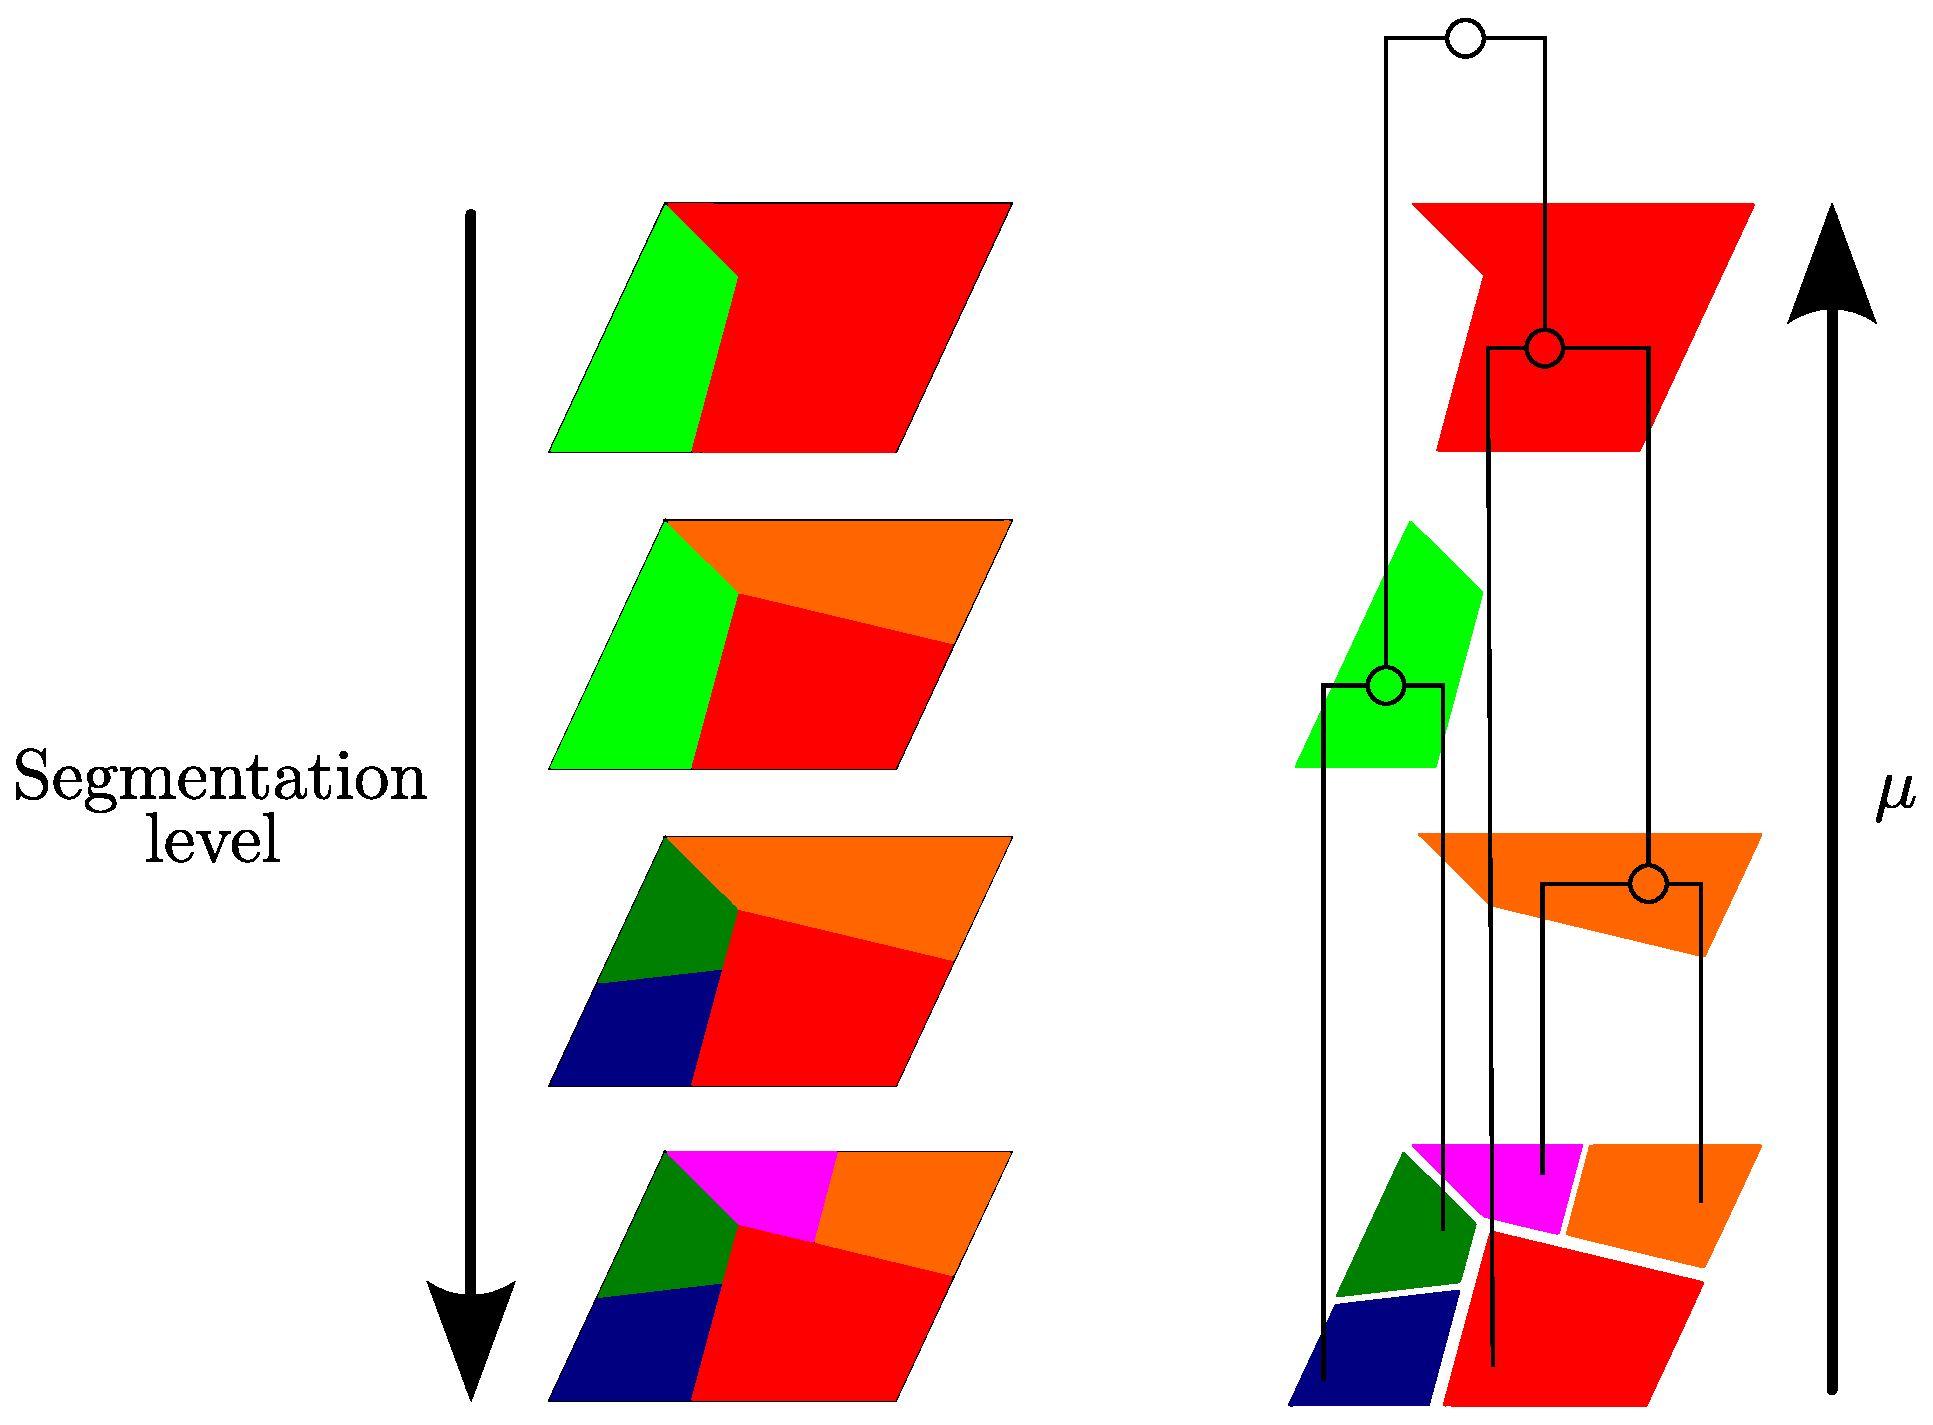
\includegraphics[width=0.5\textwidht]{Figures/seg_hierar}
%\end{figurethesis}

\begin{figurethesis}{test}
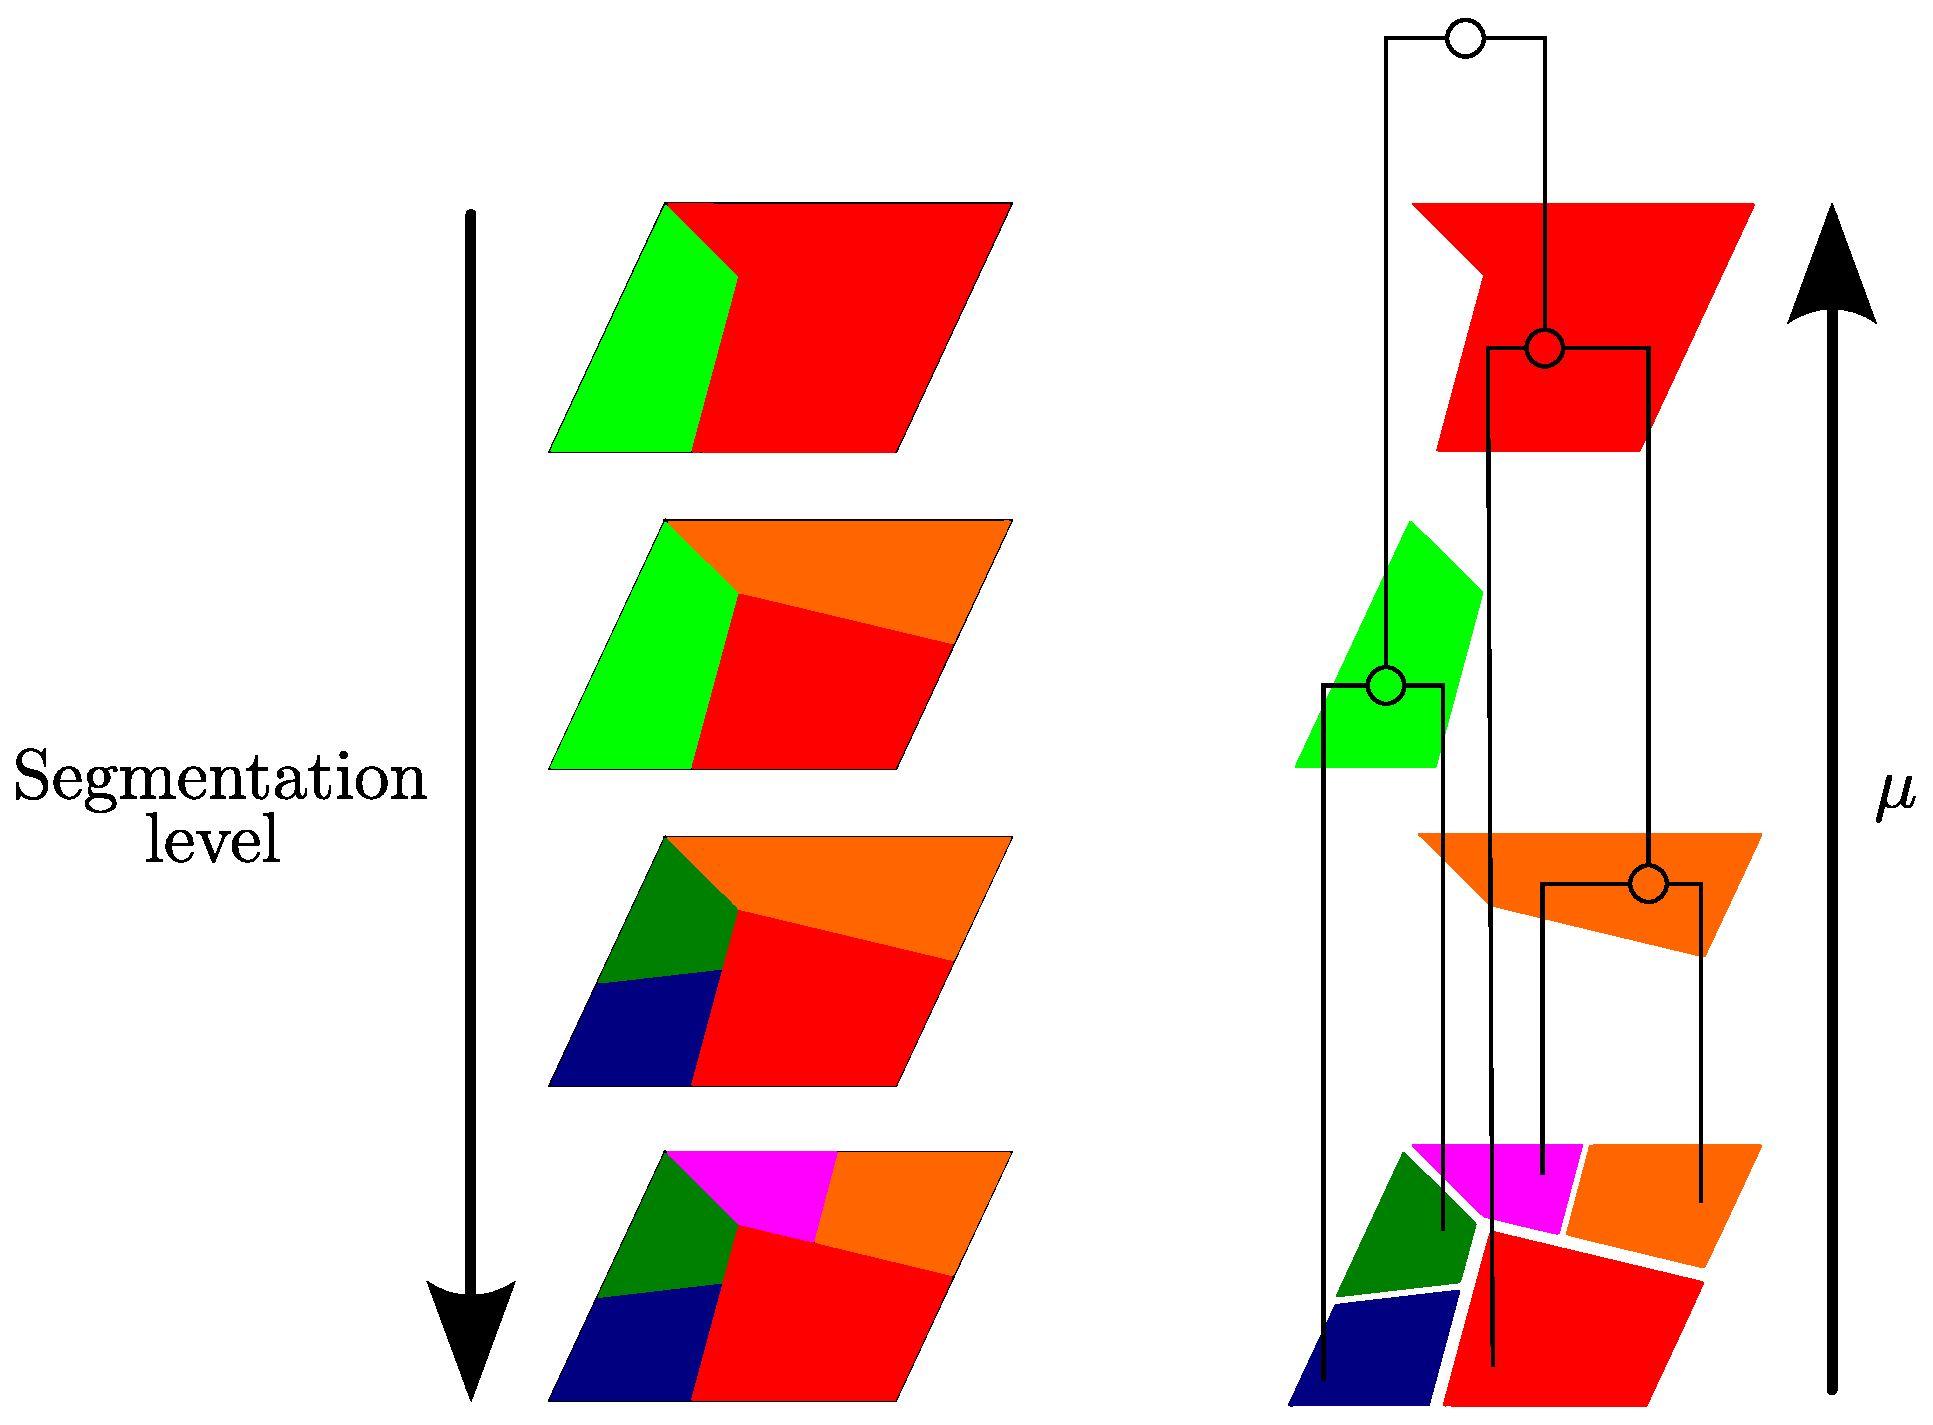
\includegraphics[width=0.75\textwidth]{Figures/seg_hierar}
\caption{Graphical depiction of concepts related to hierarchical segmentation. The diagram on the left shows partitions of an image at four different scales $\mu$. The partition at the top has the highest $\mu$ and is therefore the coarsest, the partition at the bottom is the finest.}
\label{fig:seg_hierar}
\end{figurethesis}


\subsection{Superpixels methods}
Several superpixels algorithms have been developed \citep{achanta2012slic}. They group pixels into perceptually meaningful atomic regions. Many traditional segmentation algorithms have been employed with more or less success to generate superpixels \citep{shi2000normalized, felzenszwalb2004efficient, comaniciu2002mean, vedaldi2008quick, vincent1991watersheds}. These algorithms produce satisfactory results, however, they may be relatively slow and the number, size and shape of the superpixels might not be specified. \\

Superpixels algorithms have then been developed. One can control the number of superpixel, their size and their shape. \cite{moore2008superpixel} creates superpixels based on a grid. Optimal path are found using graph cut methods. \cite{veksler2010superpixels} proposes a generation of superpixels based on a global optimization. They are obtained by stitching together overlapping image patches such that each pixel belongs to only one of the overlapping regions. \cite{levinshtein2009turbopixels} generate superpixels by a dilatation of a set of seed locations using level-set geometric flow. Resulting superpixels are constrained to have uniform size, compactness, and boundary adherence. Finally, \cite{achanta2012slic} proposes a generation of superpixels based on the k-means algorithms. A weighted distance that combines color and spatial proximity is introduced in order to control the size and the compactness of the superpixels.


\subsection{Segmentation of point cloud}
The segmentation of point cloud has been highly assessed \citep{nguyen20133d}. The aim is to extract meaningful objects. Such extraction has two principal objectives:
\begin{itemize}
\item Objects are detected so as to ease or strengthen subsequent classification task. A precise extraction is not mandatory since the labels would be refined after.
\item Objects are precisely delineated in order to derive features from these objects. A high spatial resolution is therefore expected.
\end{itemize}

In forested areas, the only reliable objects to extract are trees. The first way to extract trees from lidar data is to rasterize the point cloud and use image-based segmentation techniques to obtain trees. Several methods have been developed for single tree delineation \citep{dalponte2014tree, vega2014ptrees, kandare2014new}. 

\section{Classification}
A classification is a process that aims to categorize observation. The idea is to assign an observation to one or more classes. This can be done manually or automatically. The classification can be unsupervised, the classes need to be learned and the observation assigned. Such classification is similar to segmentation (see section \ref{sec:C1_seg}). The classification can be supervised, the target classes are known and observations with labels are available.

\subsection{Supervised classification}
A great number of supervised classification algorithms have been developed and used for remote sensing issues \citep{landgrebe2005signal, lu2007survey, mather2016classification}. There are two kind of algorithms: the parametric (or generative) and the non-parametric (or discriminative) methods.

The parametric method assume that each class follow a specific distribution (mainly gaussian). The parameters of the distribution are estimated using the learning set. This is the case for the maximum likelihood \citep{strahler1980use}, maximum a posteriori \citep{fauvel2015fast} or in \cite{trias2005high}.

The non parametric methods do not make any assumption on the classes distribution. In this category of algorithms, the most popular are the Support Vector Machines (SVM) \citep{boser1992training, scholkopf2001learning} and the Random Forest (RF) \citep{breiman2001random}. The artificial neural networks are also efficient algorithms \citep{hepner1990artificial, atkinson1997mapping}. However, despite their great performance in terms of accuracy, they have several drawbacks: firstly, the training process is time consuming and good GPU cards or specific architectures are required in order to reach decent training times \citep{dean2012large, moritz2015sparknet}. Secondly, it requires an important amount of training data in order to correctly optimize the large number of parameters (e.g., hundred of millions). Simpler methods exist, such as the k-nearest neighbor \citep{indyk1998approximate} or the decision trees \citep{breiman1984classification}. The non parametric methods are more efficient  for the discrimination of complex classes \citep{paola1995review, foody2002status}, and are considered as a basis for land cover classification \citep{camps2009kernel}.

We chose to use the RF, which besides their widespread use, since they also offer the possibility of obtaining the probability of belonging of a pixel to a class. This posterior probabilities can be then integrated into a smoothing process. They also report good results, similar to SVM (see Chapter~\ref{Chapter3}). The RF are described in section~\ref{sec:RF}.

\subsection{Random Forest}
\label{sec:RF}
The RF have been introduced by \cite{breiman2001random} and are defined by the aggregation of predictors (decision trees). Here, we refer to the RF with random inputs proposed in \cite{breiman2001random}.

The idea is to create an ensemble of samples $\mathcal{S}_{n}^{\Theta_{1}}$, ..., $\mathcal{S}_{n}^{\Theta_{k}}$ from an initial training set. A Classification and Regression Tree (CART) \citep{breiman1984classification} is built on each sample $\mathcal{S}_{n}^{\Theta_{i}}$. Each tree is built using a a random pool of $m$ features among the $M$ available features. The final classification is obtained by majority vote; each tree votes for a class and the class reaching the most votes wins (see Figure \ref{fig:RF_method}). This algorithm has two parameters: the number of trees $k$ and the number of features $m$ used to build a tree. The first parameter is arbitrary fixed to a high value. The second is generally fixed to the square root of the total number of feature \citep{gislason2006random}.

\begin{figure}[htbp]
\begin{center}
\begin{tikzpicture}
	[shape=circle,cap=round,scale=1]
	%
	\draw (0,2.5)  node[myNodeIGNGris] (data) {Dataset};
	\draw (-4,0.5)  node[myNodeIGNVert] (bootstrap1) {$\mathcal{S}_n^{\Theta_1}$};
	\node (ldots) at (0,0.5) {\textbf{\ldots}};
	\draw (4,0.5) node[myNodeIGNVert] (bootstrapN) {$\mathcal{S}_n^{\Theta_k}$};	
	
	\draw[thick,color=gray,rounded corners](-6.75,-5)--(-6.75,-1)--(-1.25,-1)--(-1.25,-5)--cycle;
	\node[color=gray] at (-5.25,-1.5) {CART 1};
	\node (first tree) at (-4,-3) {\tikz{%
	\node[draw,top color=blue!10,bottom color=blue,minimum size=6pt,circular drop shadow] {} 
	 child  foreach \A in {red,red,red}{  
	   node[draw,top color=\A!10,bottom color=\A,minimum size=4pt,circular drop shadow] {} 
	     child foreach \B in {green,green}{
	       node[draw,top color=\B!10,bottom color=\B,minimum size=3pt,circular drop shadow] {} 
	    }%
	 };%
	}};%
	
	\draw[thick,color=gray,rounded corners](1.25,-5)--(1.25,-1)--(6.75,-1)--(6.75,-5)--cycle;
	\node[color=gray] (cartk) at (2.75,-1.5) {CART K};
	\node (second tree) at (4,-3) {\tikz{%
	\node[draw,top color=blue!10,bottom color=blue,minimum size=6pt,circular drop shadow] {} 
	 child  foreach \A in {red,red,red}{  
	   node[draw,top color=\A!10,bottom color=\A,minimum size=4pt,circular drop shadow] {} 
	     child foreach \B in {green,green}{
	       node[draw,top color=\B!10,bottom color=\B,minimum size=3pt,circular drop shadow] {} 
	    }
	 };
	}};
	
	\draw (0,-6.5)  node[myNodeIGNGris] (vote) {Majority vote};
	
	\draw[myArrowIGNGris] (data.south) -- (0,1.5) -- (-4,1.5)  -- (bootstrap1.north);
	\draw[myArrowIGNGris] (data.south) -- (0,1.5) -- (4,1.5)  -- (bootstrapN.north);
	
	\draw[myArrowIGNGris] (bootstrap1.south) -- (-4,-1);
	\draw[myArrowIGNGris] (bootstrapN.south) -- (4,-1);
	
	\draw[myArrowIGNGris] (-4,-5) -- (-4,-5.5) -- (0,-5.5)  -- (vote.north);
	\draw[myArrowIGNGris] (4,-5) -- (4,-5.5) -- (0,-5.5)  -- (vote.north);

\end{tikzpicture}
\end{center}
\caption{General diagram of the operation of the Random Forest}
\label{fig:RF_method}
\end{figure}


RF have shown better classification performances than traditional Boosting methods \citep{breiman2001random} or SVM \citep{pal2005random}. They are also able to handle big dataset with large number of feature. Furthermore, a measure of feature importance have been introduced in \cite{breiman2001random}. It allows to qualify the relevance of the feature in the classification process \citep{strobl2007bias}.

The importance of a feature $\mathbf{X}_{j}$, $j\in\{1,...,q\}$ (with $q$ the number of feature) is defined as follow. Let $\mathcal{S}_{n}^{\Theta_{i}}$ be a ensemble of sample and $OOB_{i}$ all the observations that does not belong to $\mathcal{S}_{n}^{\Theta_{i}}$. $errOOB_{i}$, the error on $OOB_{i}$ using $\mathcal{S}_{n}^{\Theta_{i}}$, is then computed. A random permutation on the value of the $j^{\text{th}}$ feature of $OOB_{i}$ is performed in order to obtain $\widetilde{OOB_{i}}^j$. $err\widetilde{OOB_{i}^{j}}$ is then computed. The importance of the feature $j$, $FI(\mathbf{X_{j}})$ is the mean of the difference of the errors (see Equation \ref{eq:FI}).

\begin{equation}
\label{eq:FI}
FI(\mathbf{X_{j}})=\frac{1}{k}\sum_{i=1}^{k}(err\widetilde{OOB_{i}^{j}}-errOOB_{i})
\end{equation}
where $k$ is the number of CART.


\section{Dimension reduction and feature selection}
It is possible to derive a lot a features from the original data. All the features are used for the classification. The feature selection methods try to overcome the curse of high dimensionality \citep{bellman2015adaptive, hughes1968mean}. Indeed, the increasing number of features available tends to decrease the accuracy of the classifiers. Furthermore, the computation times increase with the number of features. Thus, reducing the feature dimension is beneficial for the classification task.

Two kind of approaches exist: first the ones based on the extraction of new features summarizing the information by the transformation of the data, generally using a projection in a space of lower dimensionality. Secondly, feature selection approaches that aim to search for an optimal subset of the features.

\subsection{Dimension reduction: feature extraction}
The most popular dimension reduction method is the Principal Component Analysis (PCA). It is an unsupervised method that aim to maximize the variance between data \citep{jolliffe2011principal}. However, it has been demonstrated that PCA is not optimal for the purpose of classification \citep{cheriyadat2003principal}. Other methods have been developed based on the PCA: the Independent Component Analysis (ICA) \citep{jutten1991blind} maximizes the statistical independence between data, and the Maximum Autocorrelation Factor (MAF) \citep{larsen2002decomposition} maximizes the spatial auto-correlation. When training samples are available, supervised methods exist, such as the linear discriminant analysis (LDA) that tries to maximize both the intra-class homogeneity and the inter-class variance \citep{fisher1936use, lebart1997multidimensional}.

\subsection{Feature selection}
Feature selection aims to search for an optimal subset of features without modifying them. To obtain such subset, one can explore the subsets of features or define a criteria to evaluate the subsets. Furthermore, the selection can be supervised or unsupervised. The first aims to discriminate the better the classes while the second are looking for an optimal subset that contains the most informative and less redundant features.
Many exploration methods for feature selection have been proposed in the literature. The naive exhaustive exploration of all the subsets can be envisaged when the number of features is not important. 

\subsubsection{Existing methods}
The feature selection methods can be separated into 3 categories: filters, wrapper and embedded. Within the filter methods, one can distinguish the supervised and unsupervised case depending on whether the notion of classes is taken into account or not.

\paragraph{\underline{$\bullet$ Filters} \\}
The filters methods use a feature selection criteria independent from the classifier. They consider the features according to their capacity to bring together elements of the same class and separate the different elements \citep{john1997enhancements} Thus, these methods compute an individual importance score for each feature, classify the features according to this score and keep only the best. Such scores can be computed using training sample or not. Such methods are independent from a classifier and are used as preliminary step to classification. When training samples are available, separability measures (e.g., Fisher \citep{fisher1936use}, Bhattacharrya or Jeffires-Matusia) allow to determine whether a feature or a subset of feature is well adapted to discriminate the classes \citep{bruzzone2000technique, herold2003spectral, de2005band, serpico2007extraction}. Statistical measures derived from information theory such as the divergence, the entropy or the mutual information have been proposed in the unsupervised case \citep{martinez2007clustering, le2011constrained} or supervised case \citep{battiti1994using, guo2008fast, estevez2009normalized, sotoca2010supervised, cang2012mutual}.
To summarize, criteria for filter selection methods are numerous and cover different approaches. The supervised ones, which sort features according to an individual importance score and retain only the $n$ best remain limited since they do not take into account the dependencies between the selected features. Approaches that directly associate relevance scores with feature sets are more interesting. A distinction is made between supervised and unsupervised approaches. The unsupervised criteria are interesting, but present a risk of selecting attributes that would not all also be useful for classification.

\paragraph{\underline{$\bullet$ Wrapper} \\}
The wrapper methods weight the features according to their pertinence for the prediction \citep{kohavi1997wrappers}. This weighting is related to the performance of a classifier.  \cite{estevez2009normalized, li2011effective, yang2007research, zhuo2008genetic} propose approaches with SVM classifiers. \cite{zhang2007dimensionality, fauvel2015fast} use maximum likelihood classifiers. The RF is also employed in \cite{diaz2006gene}. Data are separated into two subset. The first is used for the training, while the second for the evaluation. The use of a classifier is a big advantage as it fits more to the envisaged problem but can lead to overfitting. However, the use of a classifier significantly increases the computation times. Furthermore, worse results could be obtained when using a feature subset with an other classifier.

\paragraph{\underline{$\bullet$ Embedded} \\}
Eventually, the embedded methods also involve a classifier and select the features during the training process \citep{tang2014feature}. They have two advantages: since they use the data as training, they are robust. Furthermore, the feature selection and the classification are performed together, thus, they are faster than the wrapper methods. Many methods have been proposed. The RF allow to assess the feature importance \citep{breiman2001random} an is also natively embedded since the irrelevant features will not be used in the classification process. Other methods are based on the SVM classifiers, the SVM-RFE (Recursive Feature Elimination) \citep{tuia2009classification} recursively removes the less pertinent features according to a weight estimated with a SVM.

\subsubsection{Optimize the selection}
The set of possible solutions is generally too large to be visited entirely. Thus, using heuristic rules allows to find a solution close enough to the optimal solution while visiting only a reasonable number of configurations. These optimization methods can generally be distinguished in sequential or incremental methods and stochastic methods.

\paragraph{\underline{$\bullet$ Sequential approaches} \\}
The first idea is to add features step by step (forward approaches), also called Sequential Forward Selection (SFS) \citep{marill1963effectiveness}. It could also be methods that start from the entire feature set and remove feature step by step (backward approaches), also called Sequential Backward Selection (SBS) \citep{whitney1971direct}. A generalization of these methods have been proposed in \cite{kittler1978feature}. Finally, the forward and backward methods could be combined in order to improve the process. The Sequential Floating Forward Selection (SFFS) and the Sequential Floating Backward Selection (SFBS) \citep{pudil1994floating} propose such improvement. \\

\paragraph{\underline{$\bullet$ Stochastic approaches} \\}
Stochastic algorithms will involve hazard in their exploration of the space of solutions. The random initialization and search for a solution can therefore propose different solutions of equivalent quality from a single dataset.
The generation of the subset can be totally random \citep{liu1997feature}. Genetic algorithms propose a ponderation of the subsets according to their importance \citep{goldberg1989genetic}. They allow a faster convergence to a more stable solution. The Particle Swarm Optimization (PSO) algorithm \citep{yang2007research}  is also a fast and select relevant features. For finding an approximate optimal subset of features,  simulated annealing \citep{de2005band, chang2011parallel}. \\

\section{Smoothing methods}
Pixel-wise classification is not sufficient for both accurate and smooth land-cover mapping with VHR remote sensing data. This is particularly true in forested areas: the large intra-class and low inter-class variabilities of classes result in noisy label maps at pixel or tree levels. This is why various regularization solutions can be adopted from the literature (from simple smoothing to probabilistic graphical models).\\
According to \cite{SCH12}, both local and global methods can provide a regularization framework, with their own advantages and drawbacks.

\subsection{Local methods}
In local methods, the neighborhood of each element is analyzed by a filtering technique. The labels of the neighboring pixels (or the posterior class probabilities) are combined so as to derive a new label for the central pixel. Majority voting, Gaussian and bilateral filtering can be employed if it is not targeted to smooth class edges. The majority vote can also be used when a segmentation is available: the majority class is assigned to the segment.\\
The probabilistic relaxation is an other local smoothing method that aims at homogenizing probabilities of a pixel according to its neighboring pixels. The relaxation is an iterative algorithm in which the probability at each pixel is updated at each iteration in order to have it closer to the probabilities of its neighbors \citep{Gong198933}. It reports good accuracies with decent computing time and offers an alternative to edge aware/gradient-based techniques that may not be adapted in semantically unstructured environments.

\subsection{Global methods}
Global methods consider the full area of interest at the same time. They are based on Markov Random Fields (MRF, see Figure~\ref{fig:graph_cut}), the labels at different locations are not considered to be independent. The optimal configuration of labels is retrieved when finding the Maximum A Posteriori over the entire field \cite{Gab_MRF}. The problem is therefore considered as the minimization procedure of an energy $E$ over the full image $I$. Despite a simple neighborhood encoding (pairwise relations are often preferred), the optimization procedure propagates over large distances. Depending on the formulation of the energy, the global minimum may be reachable. However, a large range of optimization techniques allow to reach local minima close to the real solution, in particular for random fields with pairwise terms \cite{kolmogorov2004energy}. For genuine structured predictions, in the family of graphical probabilistic models, Conditional Random Fields (CRF, see Figure~\ref{fig:graph_cut}) have been massively adopted during the last decade. Interactions between neighboring objects, and subsequently the local context can be modeled and learned. In particular, Discriminative Random Fields (DRF, \cite{DRF}) are CRF defined over 2D regular grids, and both unary/association and binary/interaction potentials are based on labeling procedure outputs. Many techniques extending this concept or focusing on the learning or inference steps have been proposed in the literature \cite{ijcv_kohli09,Ladicky2012}. A very recent trend even consists in jointly considering CRF and deep-learning techniques for the labeling task \cite{CNN_CRF}.\\

\begin{figure}[htbp]
\begin{center}
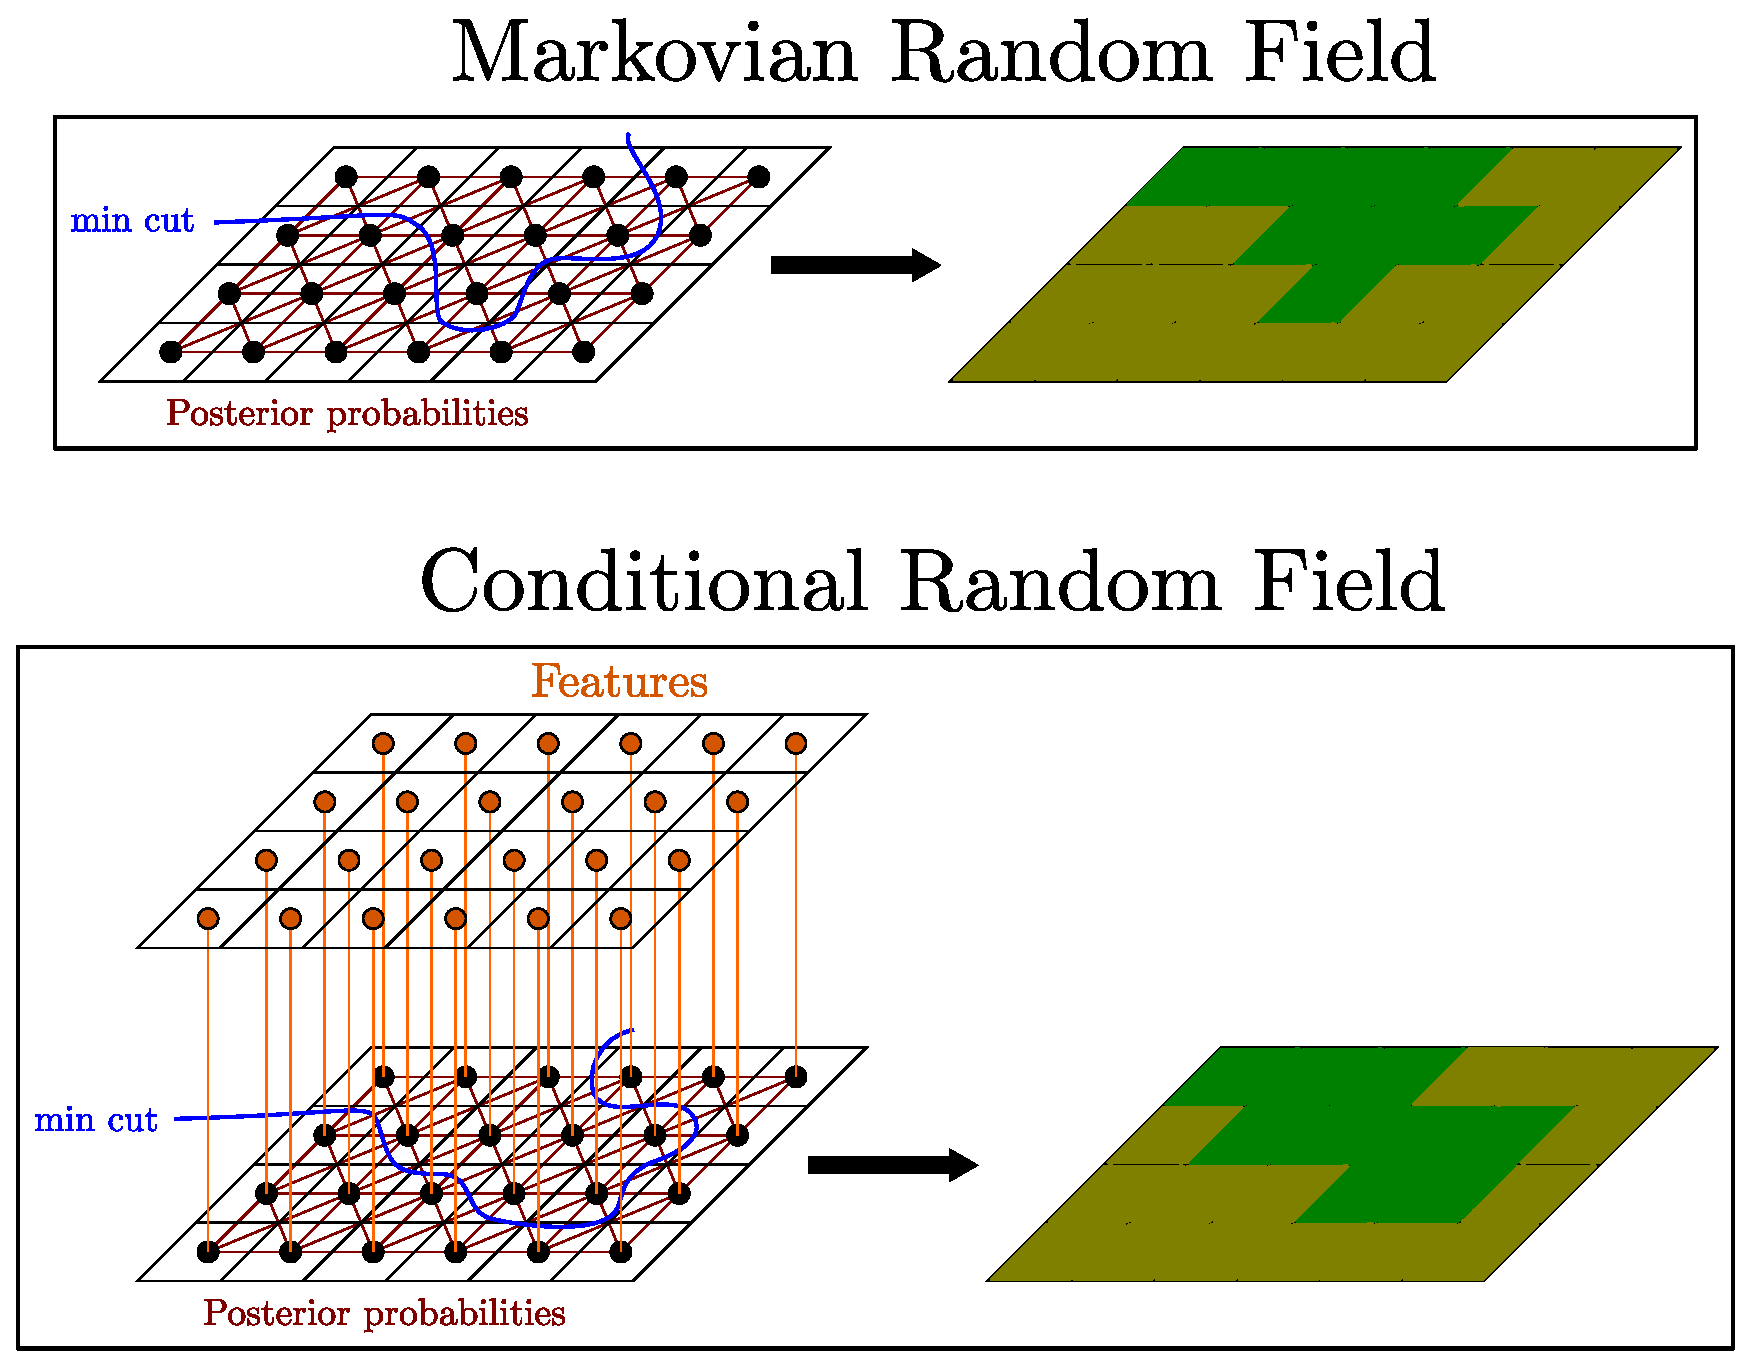
\includegraphics[width=\textwidth]{Figures/graph_cut}
\caption{8-connected MRF and CRF. The MRF only take into account the posterior probabilities to compute the graph, while CRF also include contextual information (the features).}
\label{fig:graph_cut}
\end{center}
\end{figure}

In standard LC classification tasks, global methods are known to provide significantly more accurate results \cite{SCH12} since contextual knowledge is integrated. This is all the more true for VHR remote sensing data, especially in case of a large number of classes (e.g., 10, \cite{isprs-archives-XLI-B4-11-2016}), but presents two disadvantages. For large datasets, their learning and inference steps are expensive to compute. Furthermore, parameters should often be carefully chosen for optimal performance, and authors that managed to alleviate the latter problem still report a significant computation cost \cite{Lucchi_ICCV2011}.

\stopcontents[chapters]


\openchapter
% Chapter 2

\chapter{Method} % Main chapter title
\label{Chapter2} % For referencing the chapter elsewhere, use \ref{Chapter1} 

\startcontents[chapters]
\Mprintcontents


%----------------------------------------------------------------------------------------

% Define some commands to keep the formatting separated from the content 
%\newcommand{\keyword}[1]{\textbf{#1}}
%\newcommand{\tabhead}[1]{\textbf{#1}}
%\newcommand{\code}[1]{\texttt{#1}}
%\newcommand{\file}[1]{\texttt{\bfseries#1}}
%\newcommand{\option}[1]{\texttt{\itshape#1}}

%----------------------------------------------------------------------------------------

\section{General flowchart}

With respect to the methods mentioned above, it appears that there are no forest stand segmentation method, based on tree species, that can satisfactorily handle a large number of classes ($>$5). The proposed framework is a fully automatic and modular method for species-based forest stand segmentation. The method is composed of four main steps; over-segmentation feature computation, vegetation type (mainly tree species) classification and regularization (see Figure \ref{fig:flowchart}).

\begin{figure}
\includegraphics[width=\textwidth]{Figures/method.eps}
\caption{Flowchart of the proposed method.}
\label{fig:flowchart}
\end{figure}

Features are first derived at the pixel and at the object level. The most relevant ones are subsequently selected in a supervised way. The objects are extracted using various segmentation methods, since they appear to be sufficient for subsequent steps. A classification is performed at the object level as it significantly improves the discrimination results (about $10\%$ better than the pixel-based approach). This classification is then smoothed. The smoothing may produce homogeneous vegetation type (mainly tree species) areas with smooth borders. The contributions of this method are two-fold:
\begin{itemize}
\item Such framework can be fed with specific constraints allowing to tailor the results to specific criteria (height, age, specie, maturity, density,~\ldots).
\item Here, the training set is automatically derived from an existing forest land-cover geodatabase. Specific attention is paid to the extraction of the most relevant training pixels, which is highly challenging with outdated and generalized vector databases.
\end{itemize}

\section{Over-segmentation}
The over-segmentation aims to extract small object that are consistent according to the input data. They are detected so as to ease or strengthen subsequent classification task. A precise extraction is not mandatory since the labels would be refined after.

\subsection{Segmentation of lidar data}
Two approaches could be envisaged: the direct segmentation of the point cloud or the segmentation of a rasterized lidar feature using image-based segmentation algorithms. \\

The tree extraction from the point cloud is a complex task that has been widely discussed \citep{dalponte2014tree, vega2014ptrees, kandare2014new}. However, a precise tree extraction is not needed here, since the extracted trees are only needed to improve the classification task. A coarse method is therefore adopted: the tree tops are first extracted from the lidar point clouds using a local maximum filter. A point is considered as a tree top when it has the highest height value within a 5 meter radius. Only the points above 3$\:$meters are retained as it is a common threshold of the literature \citep{eysn2012forest}, and appears to be highly discriminative in non-urban areas. Points belonging to a tree are obtained through two criteria. (i) If the height of a point within a 5$\:$m radius is greater or equal than 80\% the height of the closest tree top, it is aggregated to the tree top. (ii) If the distance in the  $(x,y)$ plane between an unlabelled point and the closest tree point is smaller than 3$\:$m  they are also aggregated. This delineation method allows to discard low vegetation, but buildings might be extracted and considered as trees. \\

The image-based segmentation are also very efficient for the over-segmentation of lidar data. They are mainly applied on the normalized digital surface model (height). Thus a method using a single band is needed. The watershed algorithm \citep{vincent1991watersheds} with specific parameters allow to obtain quickly a consistent over-segmentation of the image. A hierarchical segmentation \citep{guigues2006scale} is more adapted since only one parameter that control the segmentation level needs to be provided.

\subsection{Segmentation of optical images}

\section{Feature extraction}

\section{Classification}

\subsection{Training set design}

\subsection{Feature selection}

\subsection{Classification}

\section{Smoothing}

\subsection{Local methods}

\subsection{Global methods}

\stopcontents[chapters] 
\openchapter
% Chapter 3

\chapter{Results} % Main chapter title
\label{Chapter3} % For referencing the chapter elsewhere, use \ref{Chapter1} 

\startcontents[chapters]
\Mprintcontents

\section{Data}

\paragraph{VHR optical images \\}
The VHR images are a part of a national database. In this thesis, the images used have a spatial resolution of 50$\:$cm. Two type of ortho-images are available, a color image (3 bands; red: 600-720$\:$nm, green: 490-610$\:$nm and blue: 430-550$\:$nm) and and IRC image (3 bands; near infra-red: 750-950$\:$nm, red and green) captured by the IGN digital cameras \citep{souchon2012large}. It is then possible to obtain four band ortho-images by the combination of the two ortho-images type. \\
\paragraph{Airborne Laser Scanning \\}
IGN also process lots of flights over forested areas with a laser scanning device. The airborne lidar data were collected using an Optech 3100EA device. The footprint was 0.8$\:$m in order to increase the probability to reach the ground. The point density {for all echoes} ranges from 2 to 4$\:$points/m$^{2}$. \\
Data were acquired under leaf-on conditions and fit with the standards used in many countries for large-scale operational forest mapping purposes. \\

A prerequisite for data fusion is the most accurate alignment of the two data \citep{torabzadeh2014fusion}. A frequently used technique is to geo-rectify images using ground controls points (GCPs). A geometric transformation is established between the coordinates of GCPs and their corresponding pixels in the image. It is then applied to each pixel, so that coordinate differences on those points are reduced to the lowest possible level. This method can be easily applied and is relatively fast in terms of computation time. However the use of GCPs can still cause that the unknowns in the trajectory of the platforms produce some remarkable residual errors. Automatic methods for data registration have also been developed \citep{habib2005photogrammetric,mastin2009automatic}. \\

The registration between airborne lidar point clouds and VHR multispectral images was performed by IGN itself using ground control points. This is a standard procedure in the French mapping agency since IGN operates both sensors and has also a strong expertise in data georeferencing (this is in fact the national institute responsible for that in France for both airborne and spaceborne sensors). \\

\paragraph{National Forest Land Cover database \\}
%Le référentiel géographique forestier de l'IGN est un outil de référence pour les professionnels de la filière bois et pour les acteurs de l'environnement et de l'aménagement du territoire.
%
%La BD Forêt® est une base de données vecteur de référence pour l’espace forestier et les milieux semi-naturels. Elaborée par photo-interprétation d'images en infrarouge couleurs de la BD ORTHO®, la BD Forêt® est réalisée par emprises départementales sur le territoire métropolitain. Ce produit n'est pas disponible sur les territoires d'outre-mer.
%
%BD forêt® V1 
%
%La BD Forêt® version 1, prédécesseur de la BD Forêt® version 2, a été élaborée par photo-interprétation d’images aériennes en infrarouge couleurs.
%
%Sa surface minimale cartographiée est de 2,25 ha.
%
%La BD Forêt® version 1 présente la couverture du sol (par description de la structure et de la composition dominante des formations boisées ou naturelles) en s’appuyant sur une nomenclature départementale qui varie d’une quinzaine à une soixantaine de postes selon la diversité forestière du département cartographié.
%
%Constituée, jusqu’en 2006, par emprises départementales, elle est disponible sur l’ensemble du territoire métropolitain.
%
%Pour plus de la moitié des départements, plusieurs versions de la BD Forêt® version 1 sont disponibles.
%
%BD Forêt® V2
%
%La BD Forêt® (bd foret) version 2 est élaborée depuis 2007 par photo-interprétation d’images en infrarouge couleurs de la BD ORTHO®.
%
%Elle attribue à chaque plage cartographiée de plus de 5000m² un type de formation végétale.
%
%Ses principales caractéristiques sont les suivantes :
%
%    une nomenclature nationale de 32 postes qui repose sur une décomposition hiérarchique des critères, distinguant par exemple les peuplements purs des principales essences forestières de la forêt françaises
%    un type de formation végétale attribué à chaque plage cartographiée supérieure ou égale à 50 ares (5 000 m²)
%    une couche géométriquement compatible avec le RGE® et donc en parfaite cohérence avec la couche végétation de la BDTOPO®
%
%Réalisée par emprises départementales sur le territoire métropolitain, aujourd’hui, la BD Forêt® version 2 est disponible sur une trentaine de départements.


The IGN's forestry reference frame is a reference tool for professionals in the wood industry and for environmental and spatial planning stakeholders.

The forest LC database is a reference vector database for forest and semi-natural environments. Developed by photo-interpretation of VHR IRC optical images, The forest LC database is realized by departmental authorities in the metropolitan territory.

\paragraph{$\bullet$ Forest LC database, version 1 \\}
The version 1 of the forest LC database, was developed by photo-interpretation of aerial images in infrared colors.
Its minimum mapped surface area is 2.25 ha.
The version 1 of the forest LC database presents the soil cover (by description of the structure and the dominant composition of wooded or natural formations), based on a departmental nomenclature ranging from fifteen to sixty positions according to diversity Forestry of the mapped department.
Constituted, until 2006, at the departmental level, it is available throughout the metropolitan territory.
For more than half of the departments, several versions of the version 1 of the forest LC database are available.

\paragraph{$\bullet$ Forest LC database, version 2 \\}
The forest LC database version 2 has been developed since 2007 by photo-interpretation of VHR IRC optical images.
It assigns to each mapped range of more than 5000m$^{2}$ a type of vegetation formation.
Its main characteristics are the following:
\begin{itemize}
\item A national nomenclature of 32 posts based on a hierarchical breakdown of the criteria, distinguishing, for example, pure stands from the main forest tree species in the French forest (see Figure~\ref{fig:organigram_BD}).
\item A type of vegetation formation assigned to each mapped range greater than or equal to 50 ares (5000 m$^{2}$).
\item A layer geometrically compatible with the other vegetation layers produced by the IGN.
\end{itemize}

Produced by department in metropolitan France, the version 2 of the forest LC database in 75 (out of 95) departments.

\begin{figure}[htbp]
\begin{center}
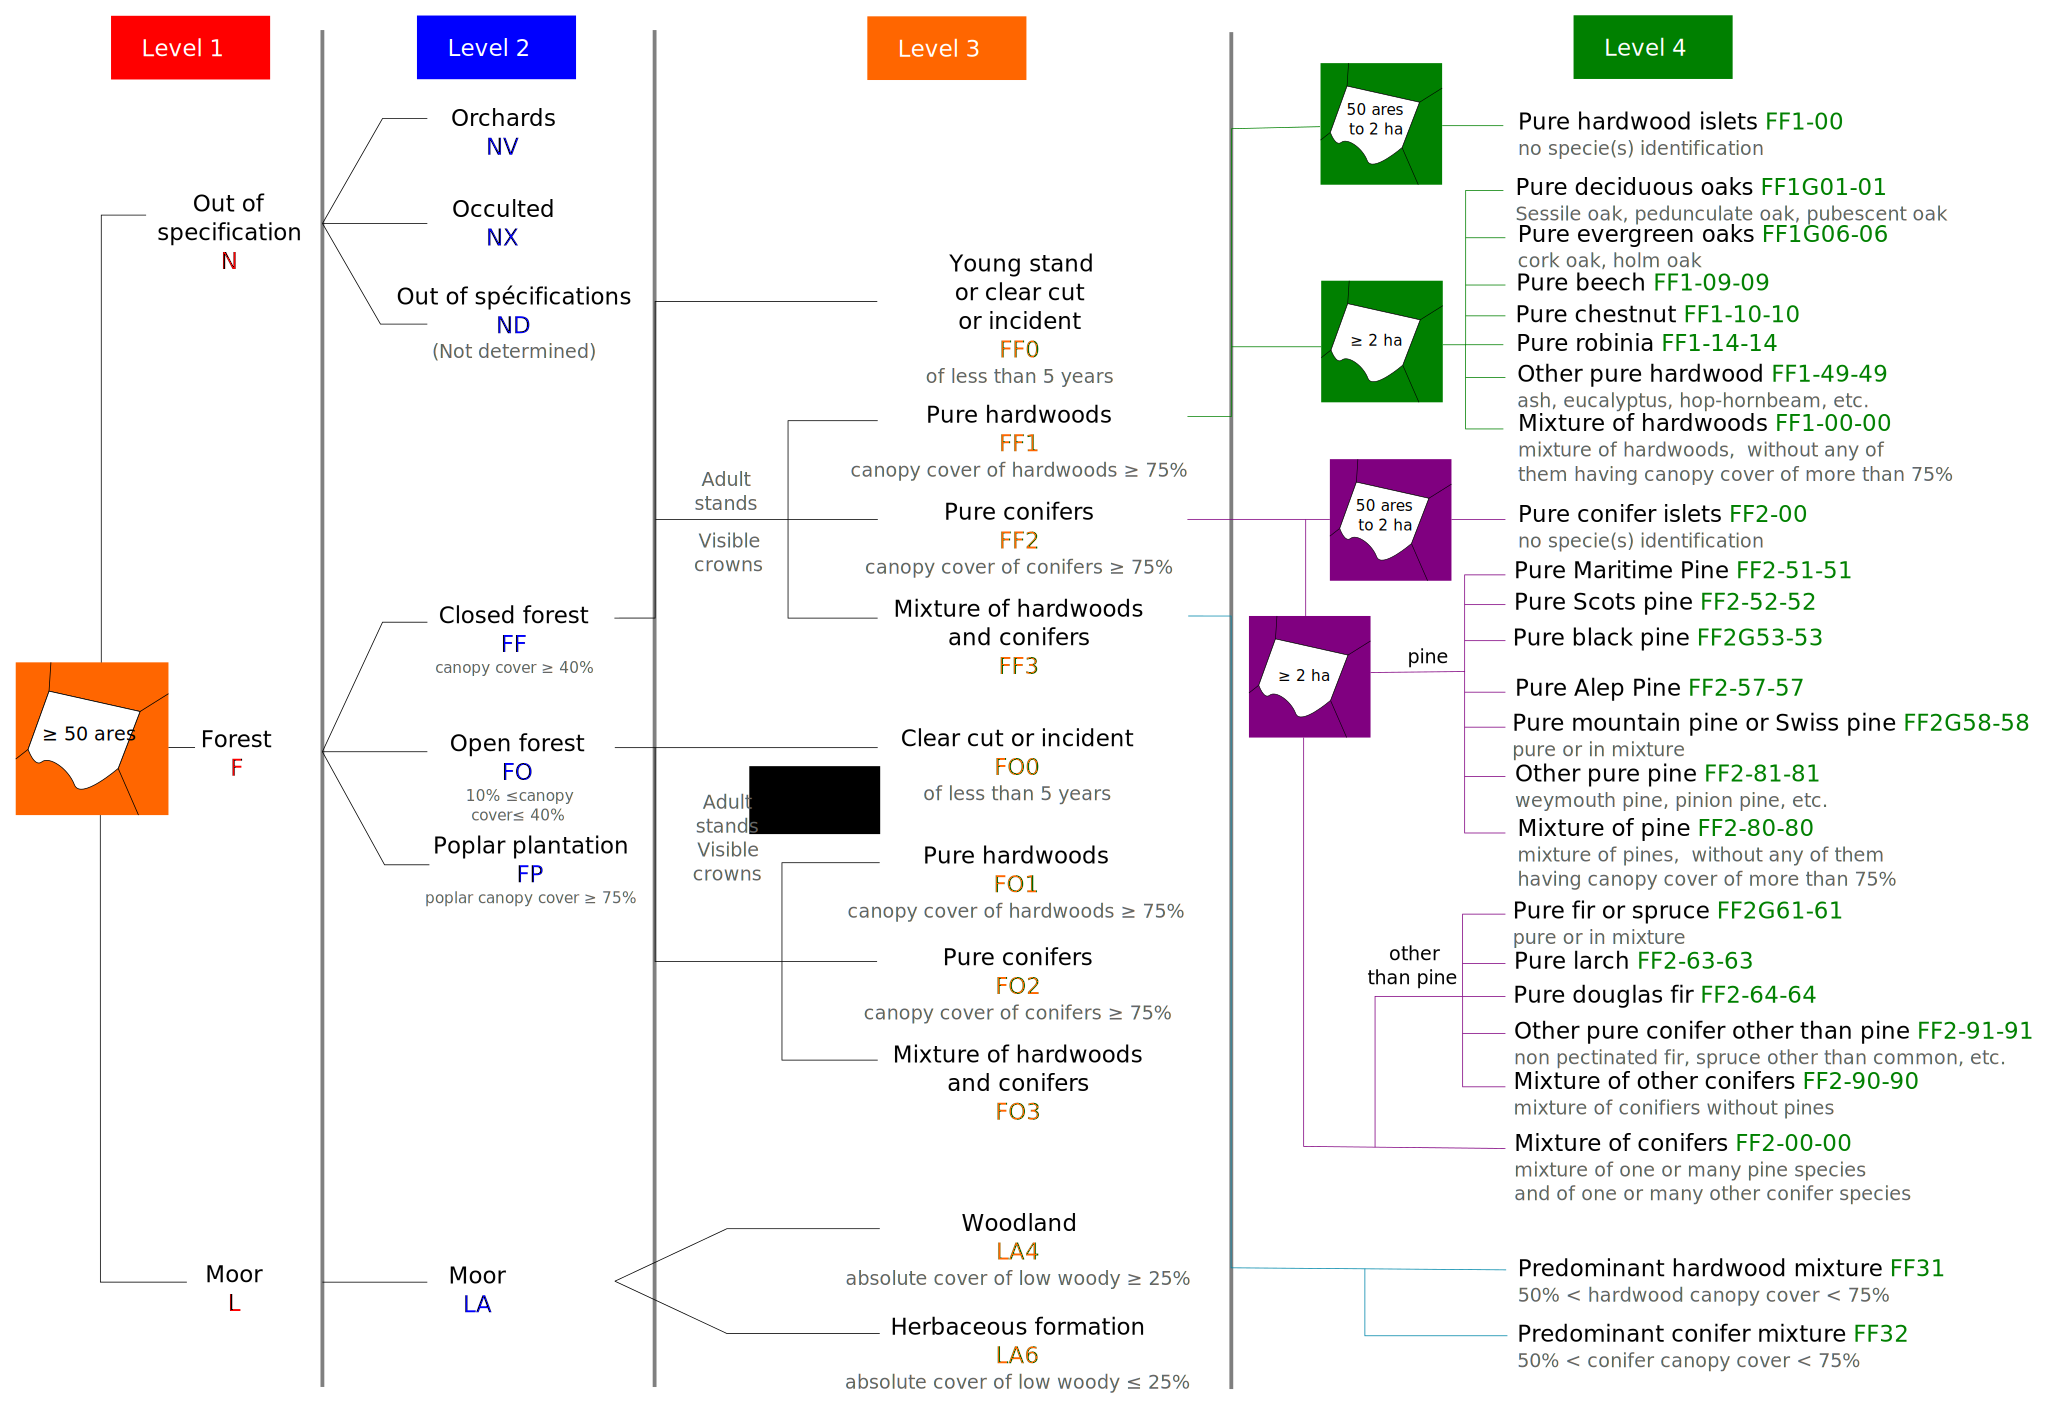
\includegraphics[width=\textwidth]{Figures/v2_organigram}
\caption{Organizational chart of the version 2 of the forest LC database.}
\label{fig:organigram_BD}
\end{center}
\end{figure}


\section{Segmentation methods}
A naive method to retrieve forest stands is to segment the input data. Such segmentation algorithms do not take into account the species information. Two algorithms were employed in order to obtain relevant stands only through the segmentation of the data.
The first segmentation algorithm is the one proposed in \cite{guigues2006scale}. It is a hierarchical segmentation algorithm that allows to control the level of segmentation through a unique scale parameter $\mu$.

The second segmentation algorithm (called PFF) employed is presented in \cite{felzenszwalb2004efficient}. It is a method for image segmentation based on pairwise region comparison considering the minimum weight edge between two regions in measuring the difference between them. 3 simples parameters need to be tuned in order to obtain relevant segmentation. $\sigma$ is the standard deviation of the gaussian filter employed to smooth the image as a pre-processing (the authors recommend $\sigma=0.8$). $k$ is a second parameter that set a scale of observation (a larger $k$ will lead to larger segments). Finally, the parameter $m$ permits to define the minimum size of a segment.

Such segmentation could allow to retrieve the stands borders easily. Furthermore, one the segmentation is performed, one can add semantic information using classification results.

These experiments have been performed only on one area presented in Figure~\ref{fig:data_direct_seg}. It is a 1$\:$km$^{2}$ area, the spatial resolution of the VHR optical image is 0.5$\:$m, and the nDSM has been rasterized at the same resolution. From these data one can see that a stand is composed of zones that are not homogeneous in term of reflectance and/or height. Furthermore, one can also note that the variability between two stands in terms of reflectance and/or height might not be important.

\begin{figure}[htbp]
\begin{center}
\begingroup
\captionsetup[subfigure]{width=0.16\textwidth}
\subfloat[VHR IRC optical image.]{
\includegraphics[width=0.3\textwidth]{Figures/C3/S2/IRC}
\label{subfig:hierar3}
}
\subfloat[nDSM.]{
\includegraphics[width=0.3\textwidth]{Figures/C3/S2/nDSM}
\label{subfig:hierar3}
}
\subfloat[Forest LC database.]{
\includegraphics[width=0.3\textwidth]{Figures/C3/S2/BD}
\label{subfig:hierar3}
}
\endgroup
\caption{VHR IRC optical image, rasterized nDSM and forest LC of the proposed area for the direct segmentation tests.}
\label{fig:data_direct_seg}
\end{center}
\end{figure}

\subsection{Retrieve stands borders}

Two strategies are employed to apply the segmentation in order to retrieve the forest stands borders from the forest LC database:
\begin{itemize}
\item The segmentation is applied to the VHR optical images, thus the resulting segment will correspond to "stands" that are homogeneous in terms of spectral reflectance. Since the optical images are employed by photo-interpreters in order to derive the forest LC, such segmentation should produce results similar to the forest LC.
\item The segmentation is also applied to the rasterized normalized digital surface model (nDSM) (canopy height without ground relief). Such segmentation would produce "stands" that are homogeneous in term of height.
\end{itemize}

The results of the segmentation of the VHR optical image using the two segmentation algorithm is presented in Figure~\ref{fig:seg_im}. In both cases, most of the borders found are not consistent with the forest LC database. Visually, the hierarchical segmentation seems to be more relevant than the PFF segmentation. However, the hierarchical segmentation produces small segments due to high variation of illumination in the image, while the PFF segments are all relatively large. 

\begin{figure}[htbp]
\begin{center}
\begingroup
\captionsetup[subfigure]{width=0.4\textwidth}
\subfloat[Hierarchical segmentation with $\mu=15$.]{
\includegraphics[width=0.45\textwidth]{Figures/C3/S2/border_hierar}
\label{subfig:hierar3}
}
\hspace*{0.05\textwidth}
\subfloat[PFF segmentation with $\sigma=0.8$, $k=500$ and $m=40000$.]{
\includegraphics[width=0.45\textwidth]{Figures/C3/S2/border_PFF_IRC}
\label{subfig:hierar3}
}
\endgroup
\caption{Result of the segmentation of the VHR optical image for the two segmentation algorithms. Blue lines correspond to the borders of the segments, red lines correspond to the borders of the forest LC.}
\label{fig:seg_im}
\end{center}
\end{figure}

The results of the segmentation of rasterized nDSM using the two segmentation algorithm is presented in Figure~\ref{fig:seg_nDSM}. Just like the segmentation of the VHR optical image, most of the borders found are not consistent with the forest LC database. Here, the PFF segmentation seems to perform better than the hierarchical segmentation visually.


\begin{figure}[htbp]
\begin{center}
\begingroup
\captionsetup[subfigure]{width=0.4\textwidth}
\subfloat[Hierarchical segmentation with $\mu=15$.]{
\includegraphics[width=0.45\textwidth]{Figures/C3/S2/border_hierar_z}
\label{subfig:hierar3}
}
\hspace*{0.05\textwidth}
\subfloat[PFF segmentation with $\sigma=0.8$, $k=500$ and $m=40000$.]{
\includegraphics[width=0.45\textwidth]{Figures/C3/S2/border_PFF_z}
\label{subfig:hierar3}
}
\endgroup
\caption{Result of the segmentation of the nDSM for the two segmentation algorithms. Blue lines correspond to the borders of the segments, red lines correspond to the borders of the forest LC.}
\label{fig:seg_nDSM}
\end{center}
\end{figure}

Since the segmentation on the VHR optical image and the nDSM does not allow to retrieve the borders from the forest LC database, different values of the parameter $\mu$ for the hierarchical segmentation on the VHR optical images (see Figure~\ref{fig:hierar}). It appears that decreasing $\mu$ does not allow to obtain the borders of the forest LC. It only leads to and over-segmentation of the image. Such over-segmentation is employed in the proposed method but is not employed as a relevant segmentation for stand delineation but as an input for object based classification.

\begin{figure}[htbp]
\begin{center}
\begingroup
\captionsetup[subfigure]{width=0.5\textwidth}
\subfloat[Hierarchical segmentation with $\mu=3$.]{
\includegraphics[width=0.45\textwidth]{Figures/C3/S2/seg_herarchical_3border_hierarchical}
\label{subfig:hierar3}
}
\hspace*{0.05\textwidth}
\subfloat[Hierarchical segmentation with $\mu=6$.]{
\includegraphics[width=0.45\textwidth]{Figures/C3/S2/seg_herarchical_6border_hierarchical}
\label{subfig:hierar6}
}
\\
\subfloat[Hierarchical segmentation with $\mu=8$.]{
\includegraphics[width=0.45\textwidth]{Figures/C3/S2/seg_herarchical_8border_hierarchical}
\label{subfig:hierar8}
}
\hspace*{0.05\textwidth}
\subfloat[Hierarchical segmentation with $\mu=10$.]{
\includegraphics[width=0.45\textwidth]{Figures/C3/S2/seg_herarchical_10border_hierarchical}
\label{subfig:hierar10}
}
\\
\subfloat[Hierarchical segmentation with $\mu=12$.]{
\includegraphics[width=0.45\textwidth]{Figures/C3/S2/seg_herarchical_12border_hierarchical}
\label{subfig:hierar12}
}
\hspace*{0.05\textwidth}
\subfloat[Hierarchical segmentation with $\mu=15$.]{
\includegraphics[width=0.45\textwidth]{Figures/C3/S2/seg_herarchical_15border_hierarchical}
\label{subfig:hierar15}
}
\endgroup
\caption{Result of the segmentation of the VHR optical image using different values of $\mu$ for the hierarchical segmentation. Blue lines correspond to the borders of the segments, red lines correspond to the borders of the forest LC.}
\label{fig:hierar}
\end{center}
\end{figure}

The two proposed segmentation algorithms are very efficient for image segmentation tasks \citep{guigues2006scale, felzenszwalb2004efficient} but are not adapted to retrieve forest stands borders. However, they can produce interesting over-segmentation since they are able to retrieve some relevant borders.

\subsection{Add semantic information}
The classification proposed in the method give information about the species at the object level. Since the segments extracted below are large than the small objects, a majority vote can be applied for each segment. The obtained label map could be compared with the forest LC.
The result of the classification for the area of interest is presented in Figure~\ref{fig:C3_S2_classif}, the confusion matrix and other accuracy metrics for this classification are presented in Table~\ref{table:C
_S2_classif}.

\begin{figure}[htbp]
\begin{center}
\begingroup
\captionsetup[subfigure]{width=0.375\textwidth}
\subfloat[Forest LC.]{
\includegraphics[width=0.45\textwidth]{Figures/C3/S2/BD}
\label{subfig:hierar3}
}
\hspace*{0.05\textwidth}
\subfloat[Classification results (overall accuracy: 81.75\%, $\kappa$:0.67).]{
\includegraphics[width=0.45\textwidth]{Figures/C3/S2/classif}
\label{subfig:hierar3}
}
\endgroup
\caption{Forest LC and classification results.}
\label{fig:C3_S2_classif}
\end{center}
\end{figure}



\section{Results of the method}
\subsection{Over-segmentation}
\subsection{Feature selection}
\subsection{Classification}
\subsection{Regularization}
\section{Co-products of the method}
\section{Semi-automatic update}
\section{Inventory}
%----------------------------------------------------------------------------------------

% Define some commands to keep the formatting separated from the content 
%\newcommand{\keyword}[1]{\textbf{#1}}
%\newcommand{\tabhead}[1]{\textbf{#1}}
%\newcommand{\code}[1]{\texttt{#1}}
%\newcommand{\file}[1]{\texttt{\bfseries#1}}
%\newcommand{\option}[1]{\texttt{\itshape#1}}

%----------------------------------------------------------------------------------------


\stopcontents[chapters] 
\openchapter
% Chapter 4

\chapter{Conclusions and perspectives} % Main chapter title
\label{Conclusion} % For referencing the chapter elsewhere, use \ref{Chapter1} 

\startcontents[chapters]
\Mprintcontents


%----------------------------------------------------------------------------------------

% Define some commands to keep the formatting separated from the content 
%\newcommand{\keyword}[1]{\textbf{#1}}
%\newcommand{\tabhead}[1]{\textbf{#1}}
%\newcommand{\code}[1]{\texttt{#1}}
%\newcommand{\file}[1]{\texttt{\bfseries#1}}
%\newcommand{\option}[1]{\texttt{\itshape#1}}

%----------------------------------------------------------------------------------------


\stopcontents[chapters]


%----------------------------------------------------------------------------------------
%	THESIS CONTENT - APPENDICES
%----------------------------------------------------------------------------------------

\appendix % Cue to tell LaTeX that the following "chapters" are Appendices

% Include the appendices of the thesis as separate files from the Appendices folder
% Uncomment the lines as you write the Appendices

\openchapter
% Appendix A

\chapter{Color code} % Main appendix title

\label{AppendixA} % For referencing this appendix elsewhere, use \ref{AppendixA}

\begin{table}
\begin{center}
\begin{tabular}{l l}
\p[l1] & {\textit{Chênes décidus}} \\
\p[l2] & {\textit{Chênes sempervirents}} \\
\p[l3] & {\textit{Hêtre}} \\
\p[l4] & {\textit{Châtaignier}} \\
\p[l5] & {\textit{Robinier}} \\
\p[l6] & {\textit{Autre feuillu pur}} \\
\p[l7] & {\textit{Pin maritime}} \\
\p[l8] & {\textit{Pin sylvestre}} \\
\p[l9] & {\textit{Pin laricio ou pin noir}} \\
\p[l10] & {\textit{Pin d'Alep}} \\
\p[l11] & {\textit{Pin à crochet ou pin cembro}} \\
\p[l12] & {\textit{Autre pin pur}} \\
\p[l13] & {\textit{Sapin ou épicéa}} \\
\p[l14] & {\textit{Mélèze}} \\
\p[l15] & {\textit{Douglas}} \\
\p[l16] & {\textit{Autre conifère pur autre que pin}} \\
\p[l17] & {\textit{Lande ligneuse}} \\
\p[l18] & {\textit{Formation herbacée}} \\
\p[l19] & {\textit{Peupleraie}} \\
\end{tabular}
\end{center}
\caption{Vegetation type color code}
\end{table}
\openchapter
% Appendix Template

\chapter{Publication} % Main appendix title

\label{Publication} % Change X to a consecutive letter; for referencing this appendix elsewhere, use \ref{AppendixX}

\startcontents[chapters]
\Mprintcontents


\section{Journal articles}

C. Dechesne, C. Mallet, A. Le Bris, V. Gouet-Brunet. \textit{Semantic segmentation of forest stands of pure species combining airborne lidar data and very high resolution multispectral imagery}. ISPRS Journal of Photogrammetry and Remote Sensing, 126 (2017), pp.129–145, 2017. \href{http://recherche.ign.fr/labos/matis/pdf/articles_revues/2017/semantic_segmentation.pdf}{\includegraphics[height=12pt]{Appendices/ic_pdf.jpg}} \\

M. Fauvel, C. Dechesne, A. Zullo, F. Ferraty. \textit{Fast forward feature selection of hyperspectral images for classification with gaussian mixture models}. IEEE Journal of Selected Topics in Applied Earth Observations and Remote Sensing, vol. 8(6), pp. 2824-2831, 2015. \href{https://arxiv.org/pdf/1501.00857v1.pdf}{\includegraphics[height=12pt]{Appendices/ic_pdf.jpg}} \\

\section{Peer-reviewed conference papers}

C. Dechesne, C. Mallet, A. Le Bris, V. Gouet-Brunet. \textit{How to combine LIDAR and very high resolution multispectral images for forest stand segmentation?} Proc. of the IEEE International Geoscience and Remote Sensing Symposium (IGARSS), Fort Worth, USA, July 2017. \href{http://recherche.ign.fr/labos/matis/pdf/articles_conf/2017/IGARSS_2017_Dechesne_Clement_final.pdf}{\includegraphics[height=12pt]{Appendices/ic_pdf.jpg}} \\

C. Dechesne, C. Mallet, A. Le Bris, V. Gouet-Brunet. \textit{Semantic segmentation of forest stands of pure specie as a global optimisation problem}. ISPRS Annals of the Photogrammetry, Remote Sensing and Spatial Information Sciences, 2017. \href{http://recherche.ign.fr/labos/matis/pdf/articles_conf/2017/workshop_hanover_2017_dechesne.pdf}{\includegraphics[height=12pt]{Appendices/ic_pdf.jpg}} \\

C. Dechesne, C. Mallet, A. Le Bris, V. Gouet-Brunet. \textit{Segmentation sémantique de données de télédétection multimodale : application aux peuplements forestiers}. ORASIS, Colleville-sur-Mer, France, Juin 2017. \href{http://recherche.ign.fr/labos/matis/pdf/articles_conf/2017/orasis2017_Dechesne.pdf}{\includegraphics[height=12pt]{Appendices/ic_pdf.jpg}} \\

C. Dechesne, C. Mallet, A. Le Bris, V. Gouet-Brunet, A. Hervieu. \textit{Forest stand segmentation using airborne Lidar data and very high resolution multispectral imagery}. International Archives of Photogrammetry, Remote Sensing and Spatial Information Sciences, vol. 41 (B3), pp 207-214 , ISPRS Congress, Prague, Juillet 2016. \href{http://recherche.ign.fr/labos/matis/pdf/articles_conf/2016/dechesne_isprs_2016.pdf}{\includegraphics[height=12pt]{Appendices/ic_pdf.jpg}} \\

\stopcontents[chapters]

%----------------------------------------------------------------------------------------
%	BIBLIOGRAPHY
%----------------------------------------------------------------------------------------

\openchapter
\setlength\bibitemsep{1.5\itemsep}
\printbibliography[heading=bibintoc]

%\renewcommand{\clearpage}{\clearpageold}
%\renewcommand{\cleardoublepage}{\cleardoublepageold}

%----------------------------------------------------------------------------------------

\end{document}  
